%\chapter{Appendices}
%\label{cha:appx}

\chapter{Detailed Derivation Process of Equations}

In Chapter~\ref{cha:dnn}, we investigated the derivative of the log-likelihood with the respect to a parameter $\theta$ in general format~(Equation~\ref{equ:part}) and in RBM~(Equation~\ref{equ:RBM}).
The following Equations~\ref{app_equ:part} and \ref{app_equ:RBM} give the detailed derivation process.
\begin{equation}
\begin{aligned}
\dfrac{\partial \log Z(\Theta)}{\partial \theta}
=&\frac{1}{Z(\Theta)}\dfrac{\partial Z(\Theta)}{\partial \theta}\\
=&\frac{1}{Z(\Theta)} \sum_{\textbf{x}} \dfrac{\partial f(\mathbf{x} \mid \Theta)}{\partial \theta} \\
=&\frac{1}{Z(\Theta)}  \sum_{\textbf{x}} f(\mathbf{x} \mid \Theta) \frac{1}{f(\mathbf{x} \mid \Theta)} \dfrac{\partial  f(\mathbf{x} \mid \Theta)}{\partial \theta} \\
=&  \sum_{\textbf{x}} \frac{f(\mathbf{x} \mid \Theta) }{Z(\Theta)} \dfrac{\partial \log f(\mathbf{x} \mid \Theta)}{\partial \theta} \\
=&  \sum_{\textbf{x}}  p(\mathbf{x} \mid \Theta) \dfrac{\partial \log f(\mathbf{x} \mid \Theta)}{\partial \theta} \\
=&\left \langle \dfrac{\partial \log f(\mathbf{c} \mid \Theta)}{\partial \theta}\right \rangle_{\mathbf{C} \sim p(\mathbf{x} \mid \Theta)}
\end{aligned}
\label{app_equ:part}
\end{equation}

\begin{equation}
\begin{aligned}
\dfrac{\partial \hat{l} (\Theta \mid \mathbf{D})}{\partial \theta} 
& = \left \langle \dfrac{\partial \log f(\mathbf{d} \mid \Theta)}{\partial \theta}\right \rangle_{\mathbf{D}} -\left \langle \dfrac{\partial \log f(\mathbf{c} \mid \Theta)}{\partial \theta}\right \rangle_{\mathbf{C} \sim p(\mathbf{x} \mid \Theta)}  \\
& = \left \langle \dfrac{\partial \log \sum_{ \mathbf{h}} e^{{-E}(\mathbf{v}, \mathbf{h} \mid \Theta)}}{\partial \theta}\right \rangle_{\mathbf{D}} 
-\left \langle \dfrac{\partial \log \sum_{ \mathbf{h}} e^{{-E}(\mathbf{v}, \mathbf{h} \mid \Theta)} }{\partial \theta}\right \rangle_{\mathbf{C} \sim p(\mathbf{v} \mid \Theta)}  \\
& = \left \langle \sum_{ \mathbf{h}} \frac{e^{{-E}(\mathbf{v}, \mathbf{h} \mid \Theta)}}{\sum_{ \mathbf{h}} e^{{-E}(\mathbf{v}, \mathbf{h} \mid \Theta)}} \cdot \dfrac{\partial {-E}(\mathbf{v}, \mathbf{h} \mid \Theta)}{\partial \theta} \right \rangle_{\mathbf{D}} 
- \left \langle \sum_{ \mathbf{h}} \frac{e^{{-E}(\mathbf{v}, \mathbf{h} \mid \Theta)}}{\sum_{ \mathbf{h}} e^{{-E}(\mathbf{v}, \mathbf{h} \mid \Theta)}} \cdot \dfrac{\partial {-E}(\mathbf{v}, \mathbf{h} \mid \Theta)}{\partial \theta} \right \rangle_{\mathbf{C} \sim p(\mathbf{v} \mid \Theta)}  \\
& = \left \langle \sum_{ \mathbf{h}} \frac{p(\mathbf{v}, \mathbf{h} \mid \Theta)}{p(\mathbf{v} \mid \Theta)} \cdot \dfrac{\partial {-E}(\mathbf{v}, \mathbf{h} \mid \Theta)}{\partial \theta} \right \rangle_{\mathbf{D}} 
- \left \langle \sum_{ \mathbf{h}}  \frac{p(\mathbf{v}, \mathbf{h} \mid \Theta)}{p(\mathbf{v} \mid \Theta)} \cdot \dfrac{\partial {-E}(\mathbf{v}, \mathbf{h} \mid \Theta)}{\partial \theta} \right \rangle_{\mathbf{C} \sim p(\mathbf{v} \mid \Theta)}  \\
& = \left \langle \sum_{ \mathbf{h}} p( \mathbf{h} \mid \mathbf{v}, \Theta) \cdot \dfrac{\partial {-E}(\mathbf{v}, \mathbf{h} \mid \Theta)}{\partial \theta} \right \rangle_{\mathbf{D}} 
- \left \langle \sum_{ \mathbf{h}} p( \mathbf{h} \mid \mathbf{v}, \Theta) \cdot \dfrac{\partial {-E}(\mathbf{v}, \mathbf{h} \mid \Theta)}{\partial \theta} \right \rangle_{\mathbf{C} \sim p(\mathbf{v} \mid \Theta)}  \\
& = \left \langle \left \langle \dfrac{\partial {-E}(\mathbf{v}, \mathbf{h} \mid \Theta)}{\partial \theta} \right \rangle_{\mathbf{D_h} \sim p( \mathbf{h} \mid \mathbf{v}, \Theta)} \right \rangle_{\mathbf{D}}
- \left \langle \left \langle \dfrac{\partial {-E}(\mathbf{v}, \mathbf{h} \mid \Theta)}{\partial \theta} \right \rangle_{\mathbf{C_h} \sim p( \mathbf{h} \mid \mathbf{c_v}, \Theta)} \right \rangle_{\mathbf{C_v} \sim p(\mathbf{v} \mid \Theta)}  \\
& = \left \langle \dfrac{\partial {-E}(\mathbf{v}, \mathbf{h} \mid \Theta)}{\partial \theta} \right \rangle_{\{\mathbf{D}, \mathbf{D}_h\} \sim p( \mathbf{h} \mid \mathbf{v}, \Theta)}
- \left \langle \dfrac{\partial {-E}(\mathbf{v}, \mathbf{h} \mid \Theta)}{\partial \theta} \right \rangle_{\{\mathbf{C_v}, \mathbf{C_h}\} \sim p( \mathbf{v}, \mathbf{h} \mid  \Theta)} \\
\end{aligned}
\label{app_equ:RBM}
\end{equation}

\chapter[More Experimental Results]{More Experimental Results for Chapter \ref{cha:sdlm}}
\label{sec:app2}
In Chapter~\ref{cha:sdlm}, Figures~\ref{fig:sols_ae} and \ref{fig:sols_rbm} show the comparisons of different solutions for reducing correlations in training spiking Autoencoders~(SAEs) and spiking Restricted Boltzmann Machines~(SRBMs).
In this section, Figures~\ref{fig:sol1_ae} to \ref{fig:sol4_rbm} present the detailed experimental results for this comparison.

To validate the learning capability of the proposed off-line training method on Leaky Integrate-and-Fire(LIF) neurons, Figures~\ref{fig:LIF_sae} and \ref{fig:LIF_srbm} demonstrate the results conducting the same experiments shown in Figures~\ref{fig:sols_ae} and \ref{fig:sols_rbm}.

In addition, to provide a closer observation of the trained weights in Figures~\ref{fig:weights_ae} and \ref{fig:weights_rbm}, the enlarged images are shown in Figures~\ref{fig:weights_ae1} to \ref{fig:weights_rbm6}.
\begin{figure}
	\centering
	\begin{subfigure}[t]{0.48\textwidth}
		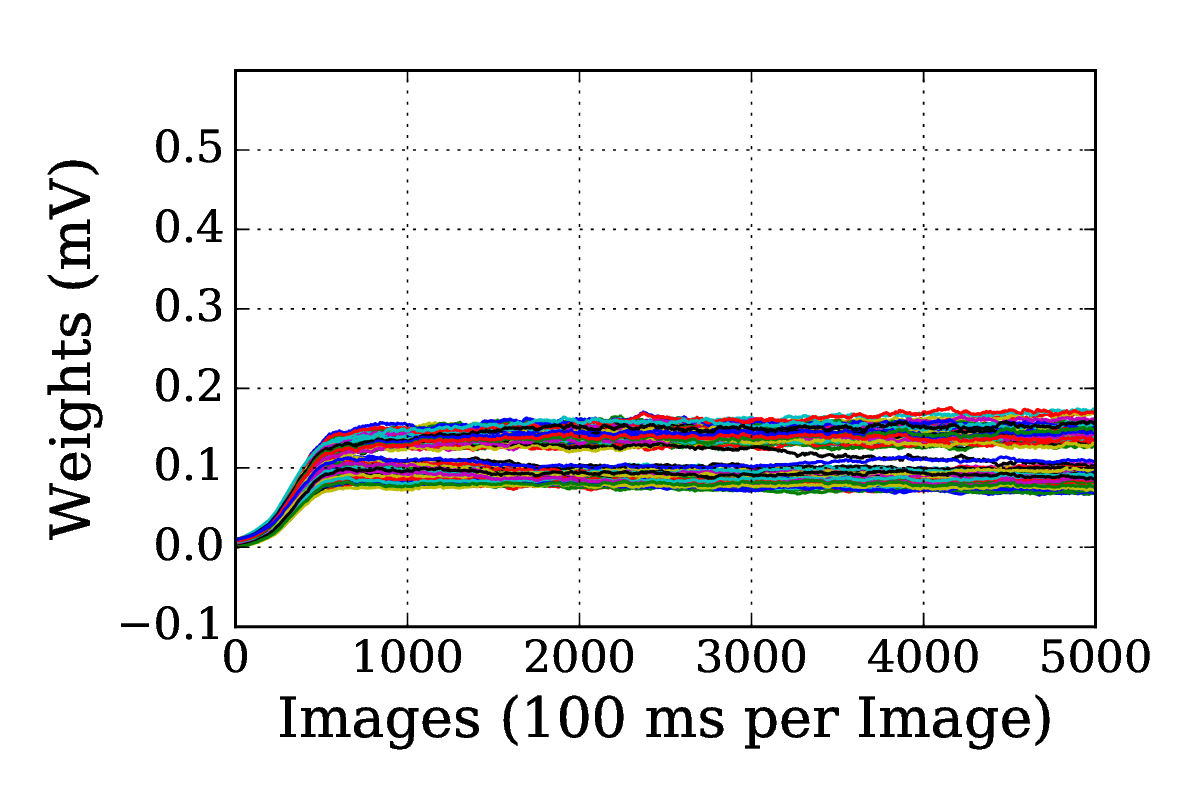
\includegraphics[width=\textwidth]{pics_sdlm/01_exp_SAE_Orig_long/exp1_weights_s.png}
		\caption{Weights of Exp1}
	\end{subfigure}
	\begin{subfigure}[t]{0.48\textwidth}
		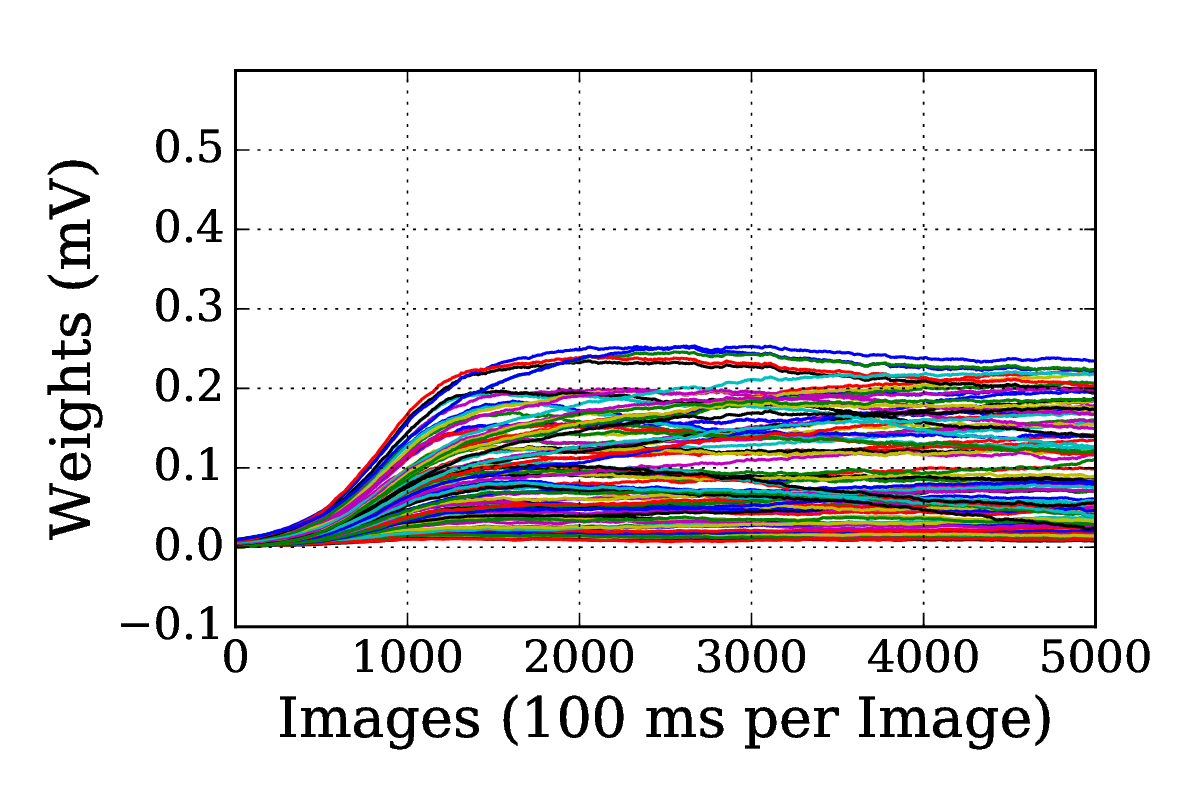
\includegraphics[width=\textwidth]{pics_sdlm/01_exp_SAE_Orig_long/exp2_weights_s.png}
		\caption{Weights of Exp2}
	\end{subfigure}
	\begin{subfigure}[t]{0.48\textwidth}
		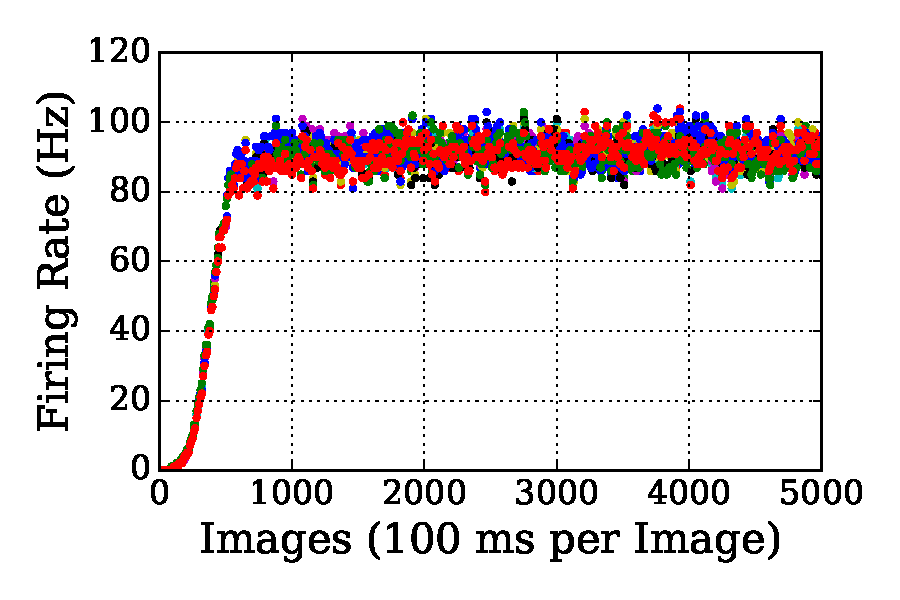
\includegraphics[width=\textwidth]{pics_sdlm/01_exp_SAE_Orig_long/exp1_recon_s.pdf}
		\caption{Reconstruction of visible units in Exp1}
	\end{subfigure}
	\begin{subfigure}[t]{0.48\textwidth}
		\includegraphics[width=\textwidth]{pics_sdlm/01_exp_SAE_Orig_long/exp2_recon_s.pdf}
		\caption{Reconstruction of visible units in Exp2}
	\end{subfigure}\\
	\begin{subfigure}[t]{0.48\textwidth}
		\includegraphics[width=\textwidth]{pics_sdlm/01_exp_SAE_Orig_long/exp1_hid_s.pdf}
		\caption{Output of hidden units in Exp1}
	\end{subfigure}
	\begin{subfigure}[t]{0.48\textwidth}
		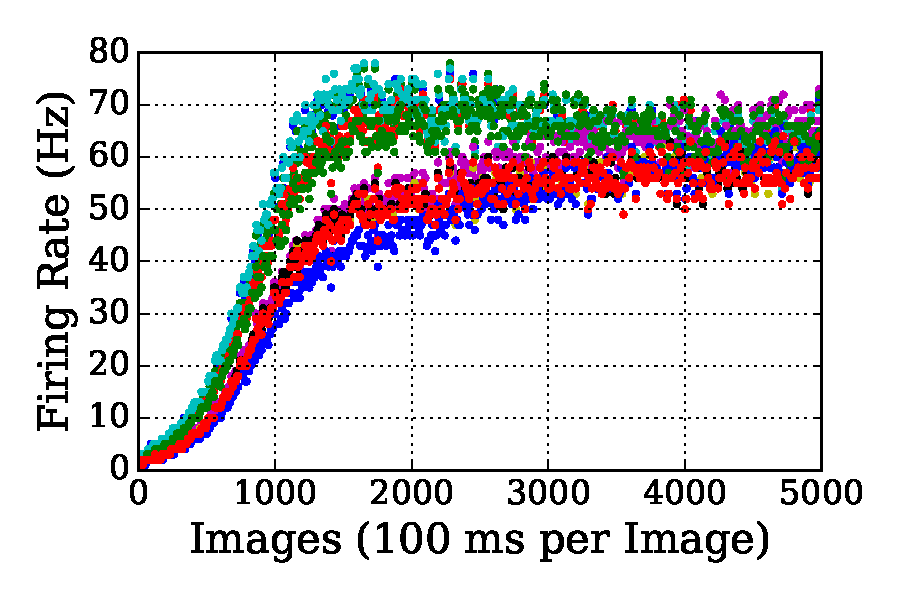
\includegraphics[width=\textwidth]{pics_sdlm/01_exp_SAE_Orig_long/exp2_hid_s.pdf}
		\caption{Output of hidden units in Exp2}
	\end{subfigure}\\
	\begin{subfigure}[t]{0.48\textwidth}
		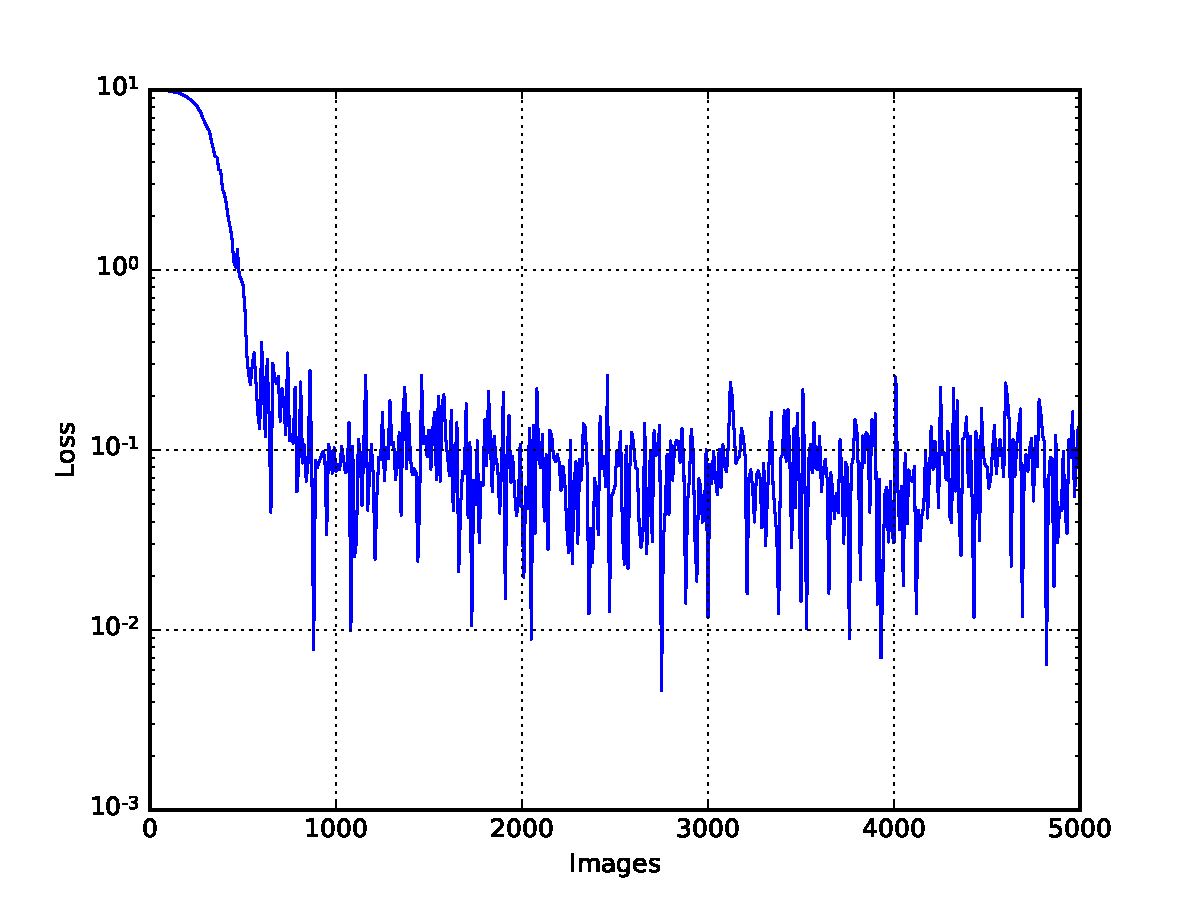
\includegraphics[width=\textwidth]{pics_sdlm/01_exp_SAE_Orig_long/exp1_mse_nons.pdf}
		\caption{Loss of Exp1}
	\end{subfigure}
	\begin{subfigure}[t]{0.48\textwidth}
		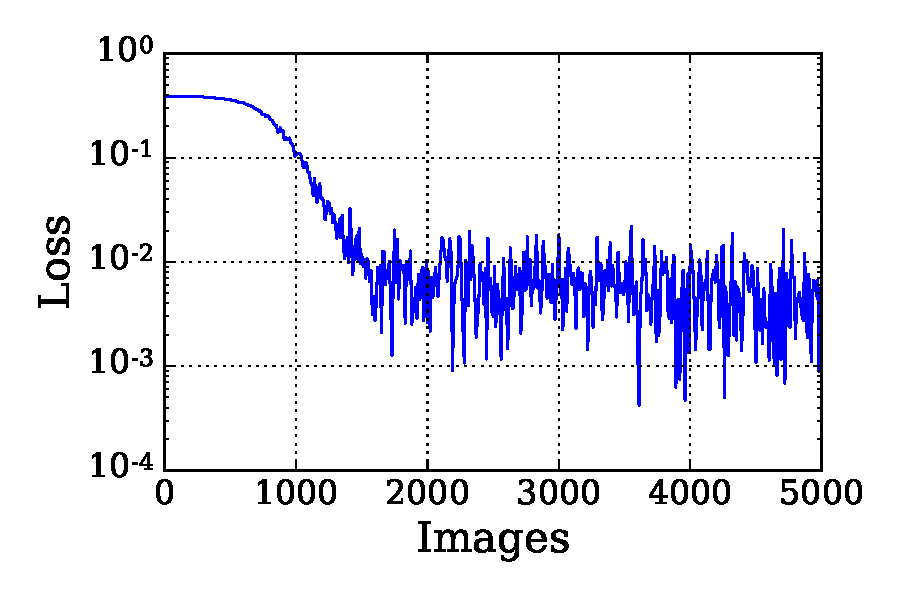
\includegraphics[width=\textwidth]{pics_sdlm/01_exp_SAE_Orig_long/exp2_mse_nons.pdf}
		\caption{Loss of Exp2}
	\end{subfigure}
	\caption{Weights and firing rates of visible and hidden units change during training of the reconstruction tests of spiking AE with Solution 1. 
		Experiments 1) 10 visible units fully connected to 10 hidden units with Poisson spike trains of 100~Hz which lasted 100~ms; 2) same network fed with 10 Poisson spike trains of firing rate ranging from 10~Hz to 100~Hz.}
	\label{fig:sol1_ae}
\end{figure}

\begin{figure}
	\centering
	\begin{subfigure}[t]{0.48\textwidth}
		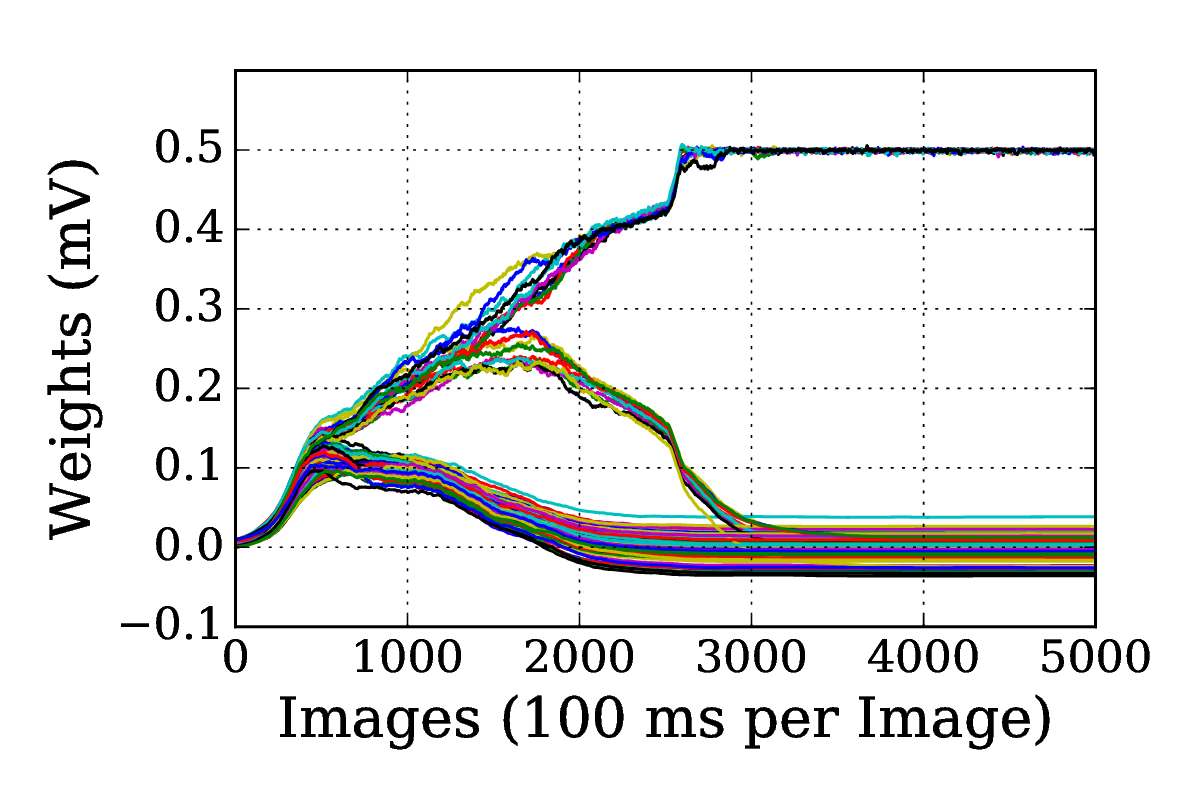
\includegraphics[width=\textwidth]{pics_sdlm/11_exp_SRBM_Orig_long/exp1_weights_s.png}
		\caption{Weights of Exp1}
	\end{subfigure}
	\begin{subfigure}[t]{0.48\textwidth}
		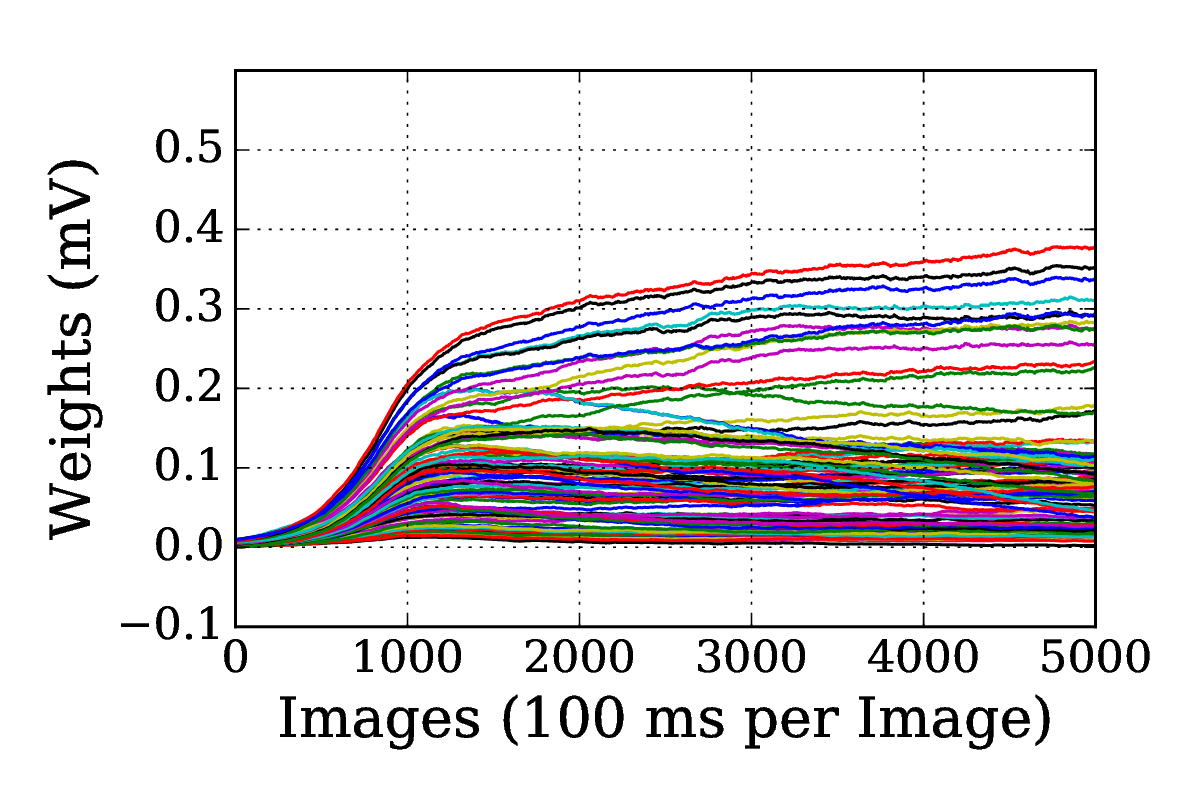
\includegraphics[width=\textwidth]{pics_sdlm/11_exp_SRBM_Orig_long/exp2_weights_s.png}
		\caption{Weights of Exp2}
	\end{subfigure}
	\begin{subfigure}[t]{0.48\textwidth}
		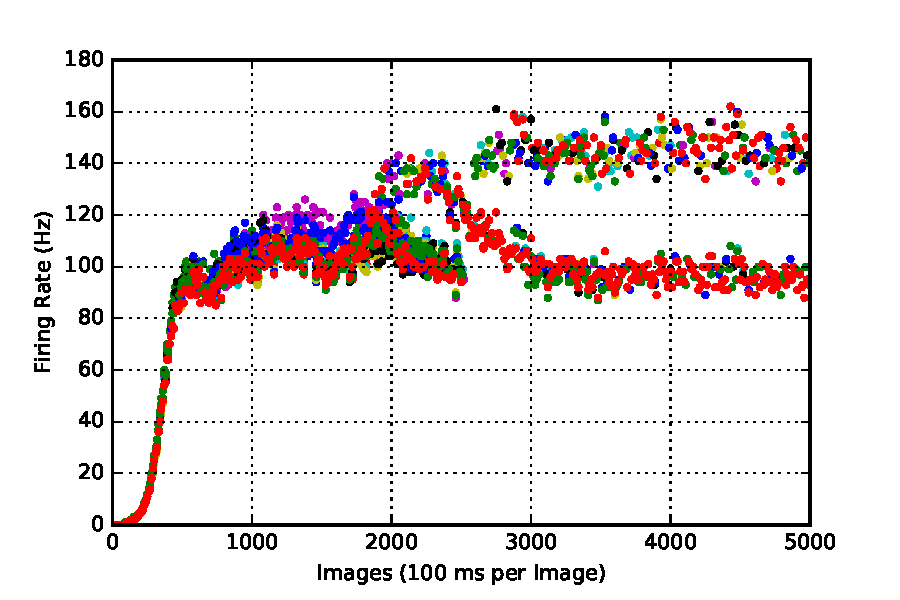
\includegraphics[width=\textwidth]{pics_sdlm/11_exp_SRBM_Orig_long/exp1_recon_s.pdf}
		\caption{Reconstruction of visible units in Exp1}
	\end{subfigure}
	\begin{subfigure}[t]{0.48\textwidth}
		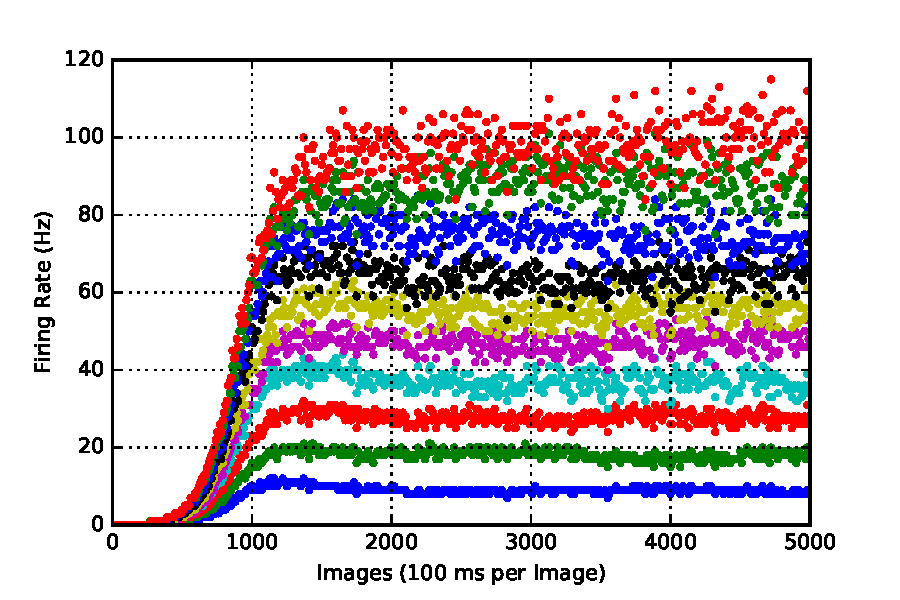
\includegraphics[width=\textwidth]{pics_sdlm/11_exp_SRBM_Orig_long/exp2_recon_s.pdf}
		\caption{Reconstruction of visible units in Exp2}
	\end{subfigure}\\
	\begin{subfigure}[t]{0.48\textwidth}
		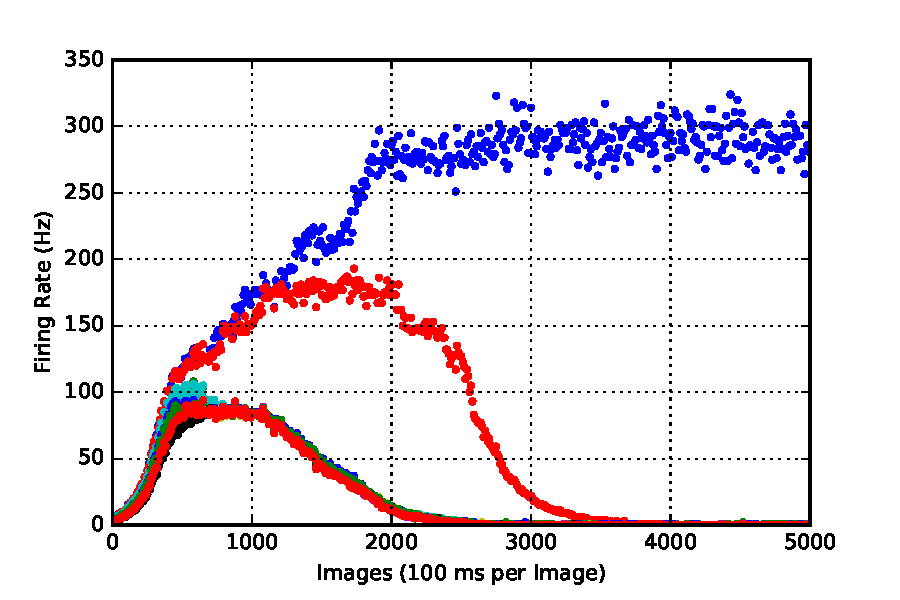
\includegraphics[width=\textwidth]{pics_sdlm/11_exp_SRBM_Orig_long/exp1_hid_s.pdf}
		\caption{Output of hidden units in Exp1}
	\end{subfigure}
	\begin{subfigure}[t]{0.48\textwidth}
		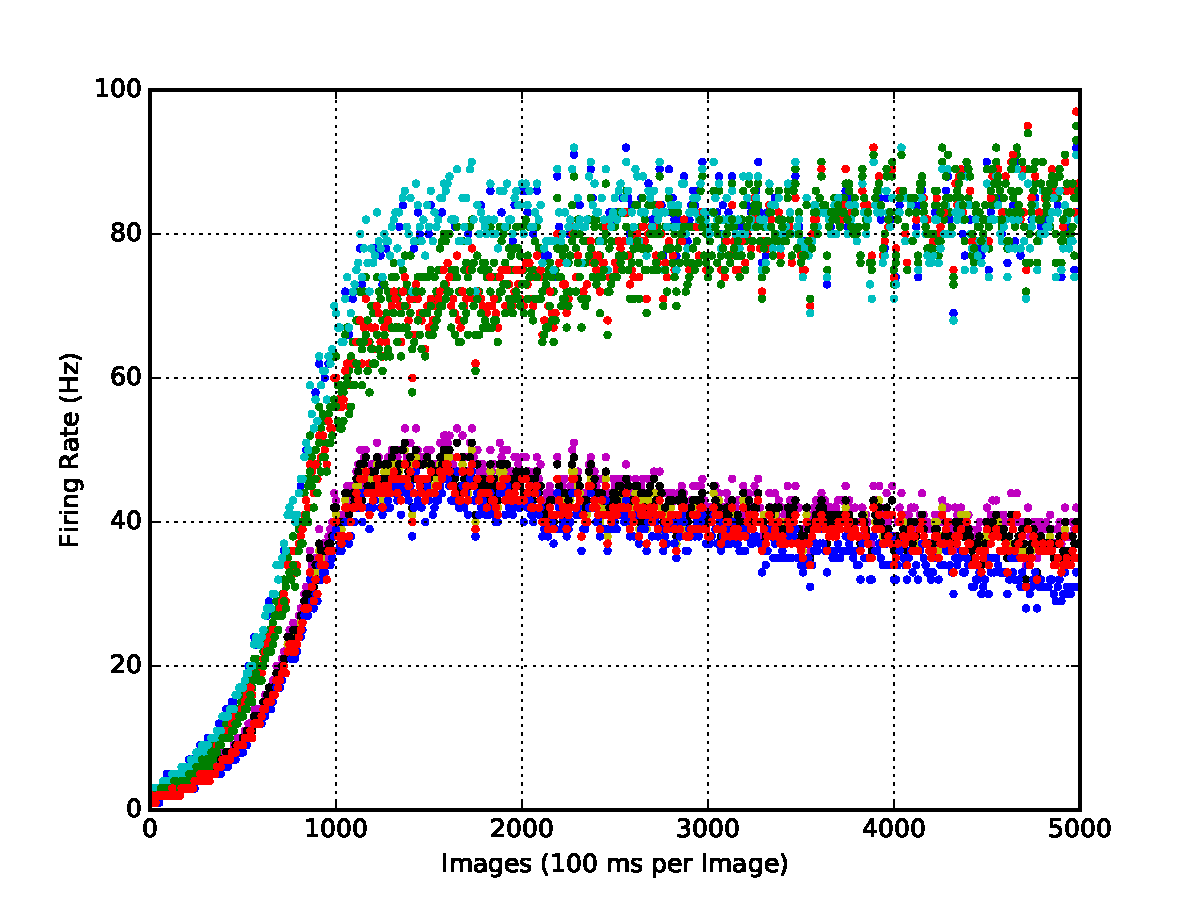
\includegraphics[width=\textwidth]{pics_sdlm/11_exp_SRBM_Orig_long/exp2_hid_s.pdf}
		\caption{Output of hidden units in Exp2}
	\end{subfigure}\\
	\begin{subfigure}[t]{0.48\textwidth}
		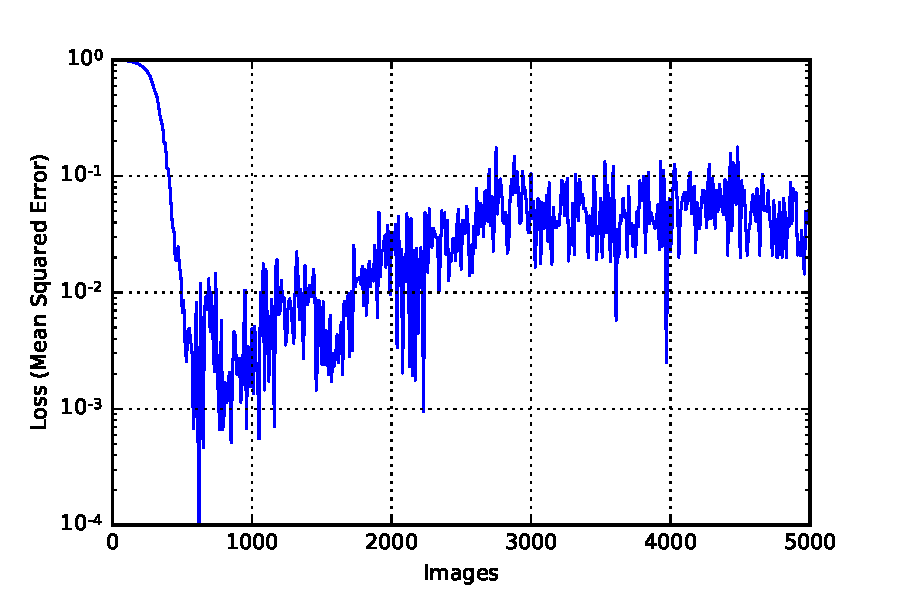
\includegraphics[width=\textwidth]{pics_sdlm/11_exp_SRBM_Orig_long/exp1_mse_nons.pdf}
		\caption{Loss of Exp1}
	\end{subfigure}
	\begin{subfigure}[t]{0.48\textwidth}
		\includegraphics[width=\textwidth]{pics_sdlm/11_exp_SRBM_Orig_long/exp2_mse_nons.pdf}
		\caption{Loss of Exp2}
	\end{subfigure}
	\caption{Weights and firing rates of visible and hidden units change during training of the reconstruction tests of spiking RBM with Solution 1. 
		Experiments 1) 10 visible units fully connected to 10 hidden units with Poisson spike trains of 100~Hz which lasted 100~ms; 2) same network fed with 10 Poisson spike trains of firing rate ranging from 10~Hz to 100~Hz.}
	\label{fig:sol1_rbm}
\end{figure}

\begin{figure}
	\centering
	\begin{subfigure}[t]{0.48\textwidth}
		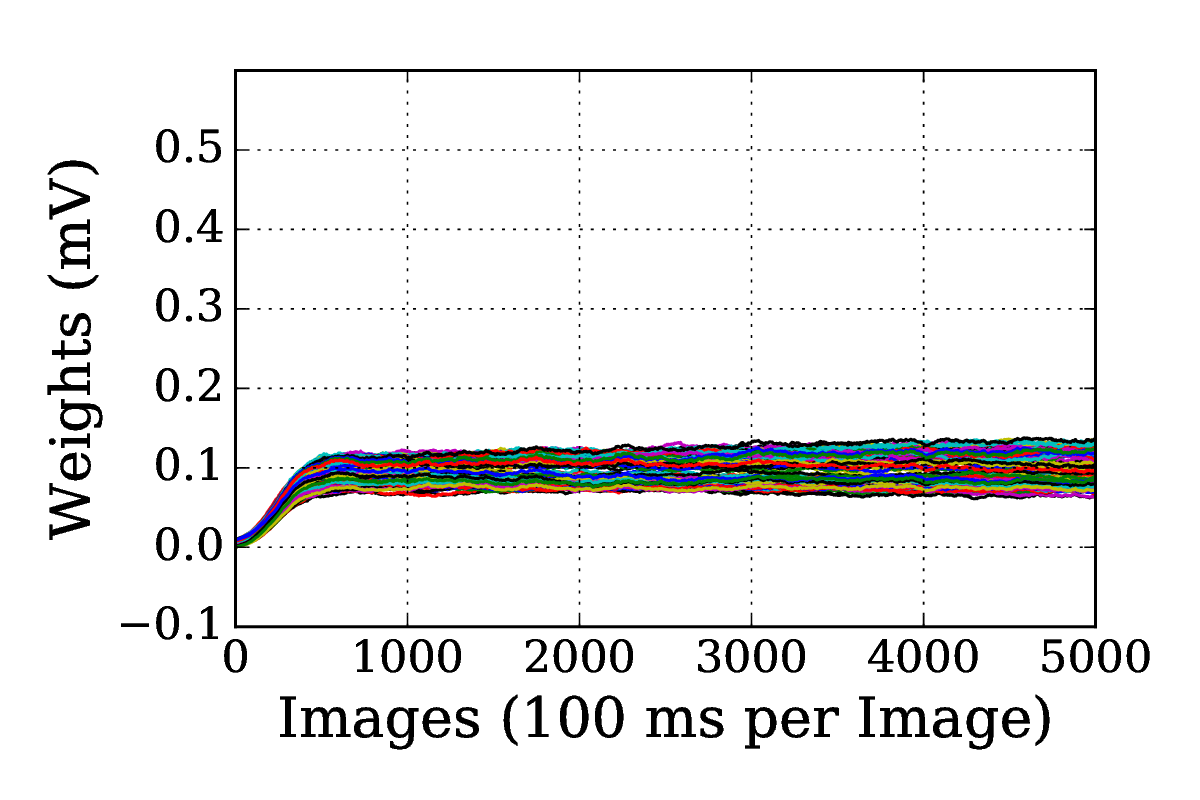
\includegraphics[width=\textwidth]{pics_sdlm/03_exp_SAE_noise_long/exp1_weights_s.png}
		\caption{Weights of Exp1}
	\end{subfigure}
	\begin{subfigure}[t]{0.48\textwidth}
		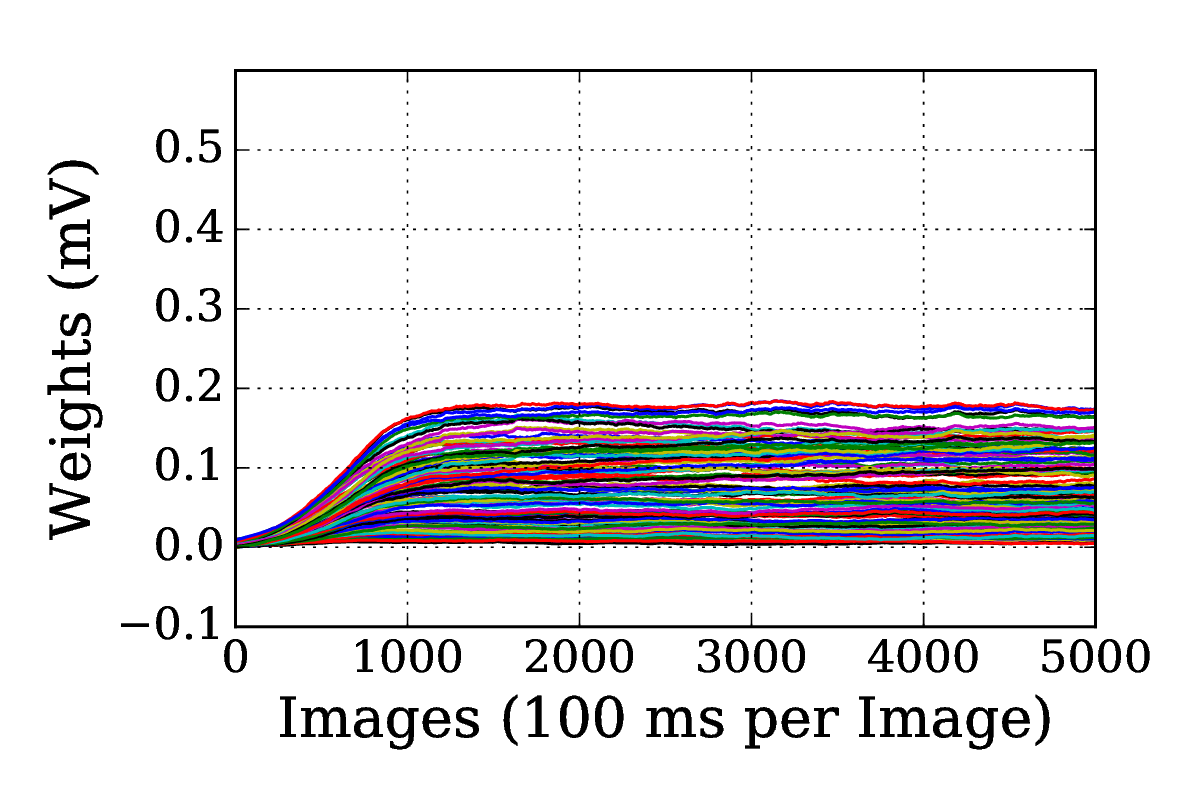
\includegraphics[width=\textwidth]{pics_sdlm/03_exp_SAE_noise_long/exp2_weights_s.png}
		\caption{Weights of Exp2}
	\end{subfigure}
	\begin{subfigure}[t]{0.48\textwidth}
		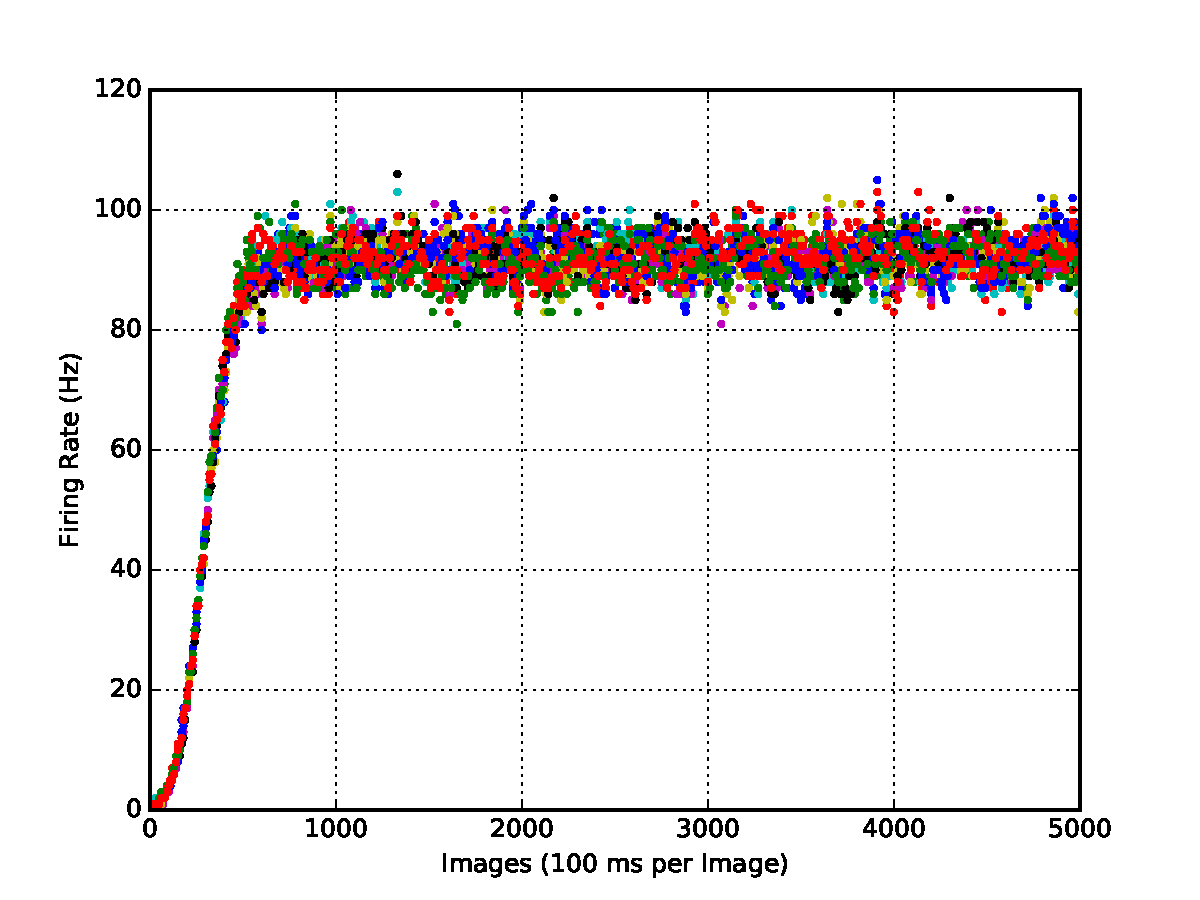
\includegraphics[width=\textwidth]{pics_sdlm/03_exp_SAE_noise_long/exp1_recon_s.pdf}
		\caption{Reconstruction of visible units in Exp1}
	\end{subfigure}
	\begin{subfigure}[t]{0.48\textwidth}
		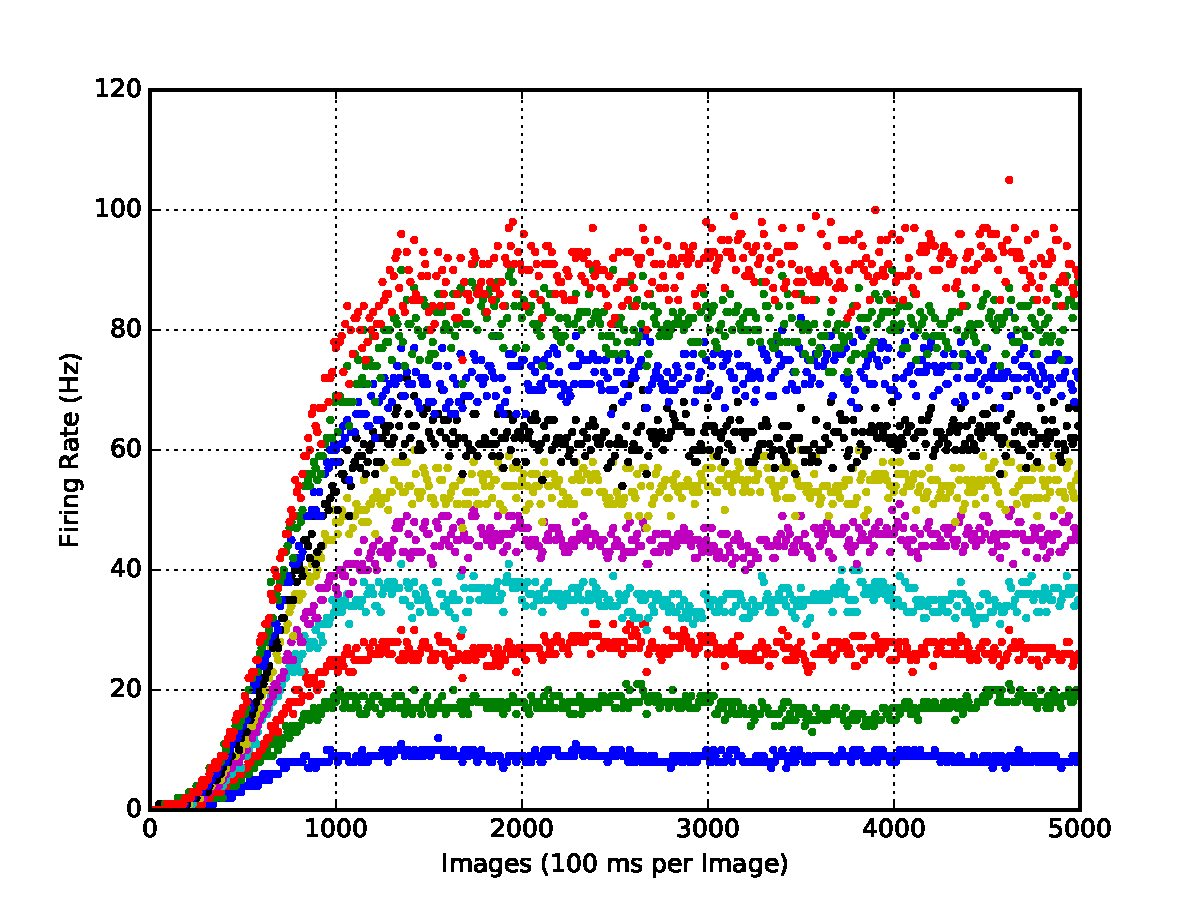
\includegraphics[width=\textwidth]{pics_sdlm/03_exp_SAE_noise_long/exp2_recon_s.pdf}
		\caption{Reconstruction of visible units in Exp2}
	\end{subfigure}\\
	\begin{subfigure}[t]{0.48\textwidth}
		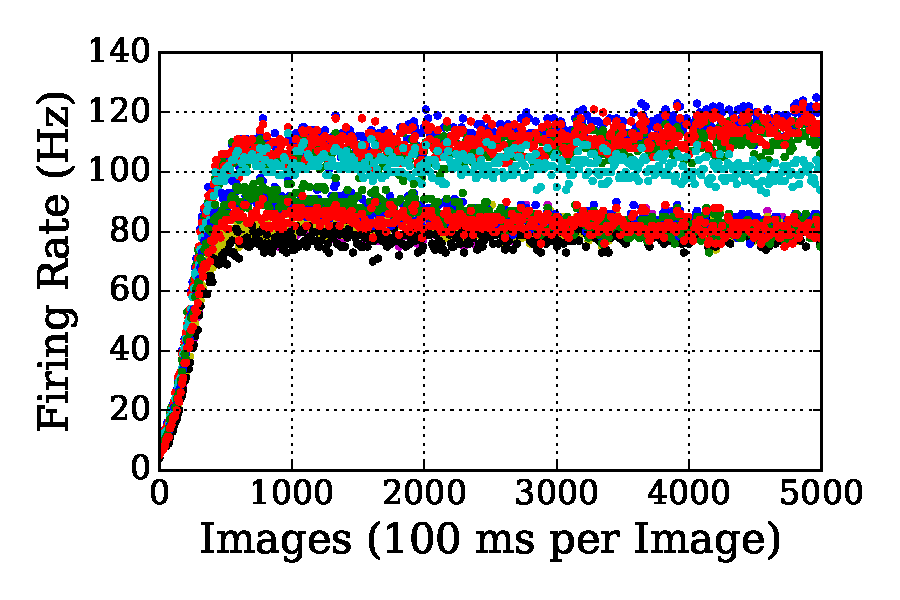
\includegraphics[width=\textwidth]{pics_sdlm/03_exp_SAE_noise_long/exp1_hid_s.pdf}
		\caption{Output of hidden units in Exp1}
	\end{subfigure}
	\begin{subfigure}[t]{0.48\textwidth}
		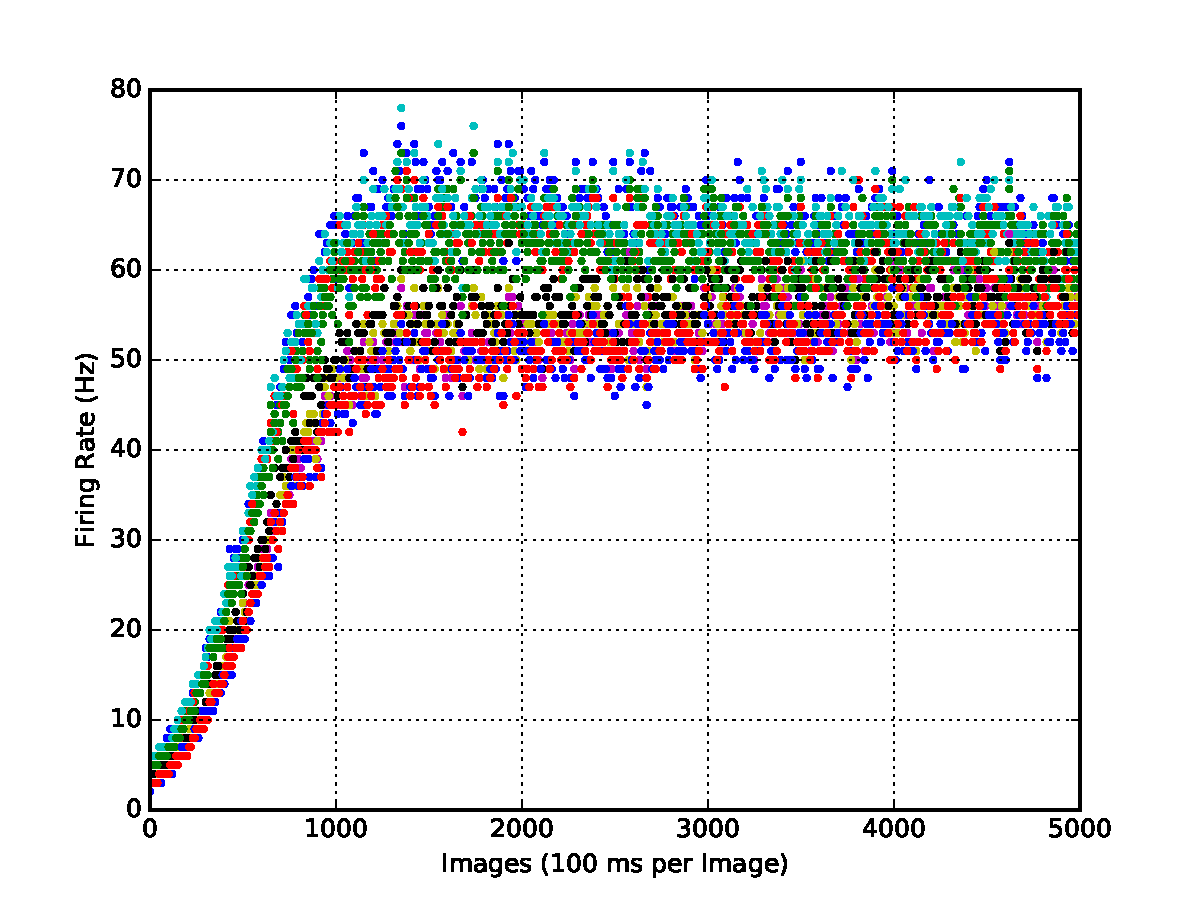
\includegraphics[width=\textwidth]{pics_sdlm/03_exp_SAE_noise_long/exp2_hid_s.pdf}
		\caption{Output of hidden units in Exp2}
	\end{subfigure}\\
	\begin{subfigure}[t]{0.48\textwidth}
		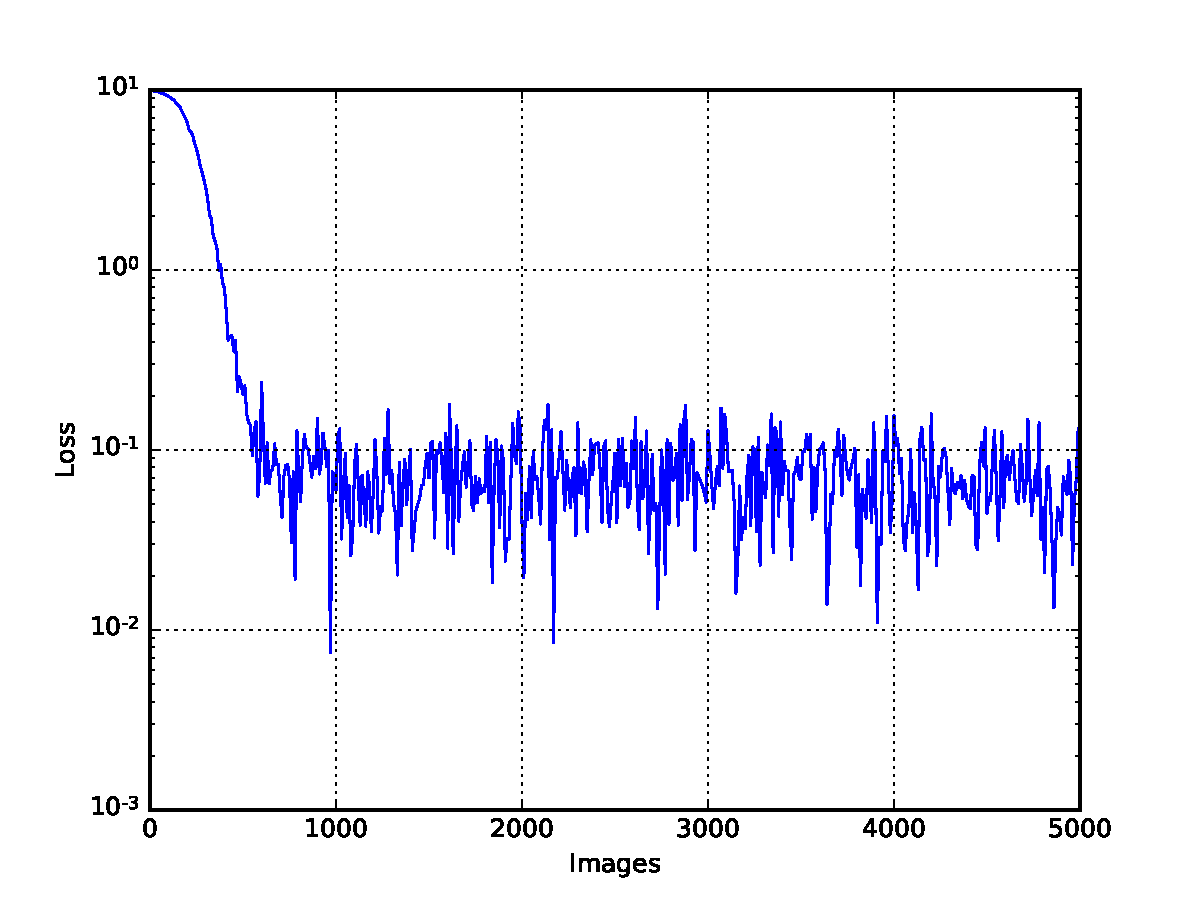
\includegraphics[width=\textwidth]{pics_sdlm/03_exp_SAE_noise_long/exp1_mse_nons.pdf}
		\caption{Loss of Exp1}
	\end{subfigure}
	\begin{subfigure}[t]{0.48\textwidth}
		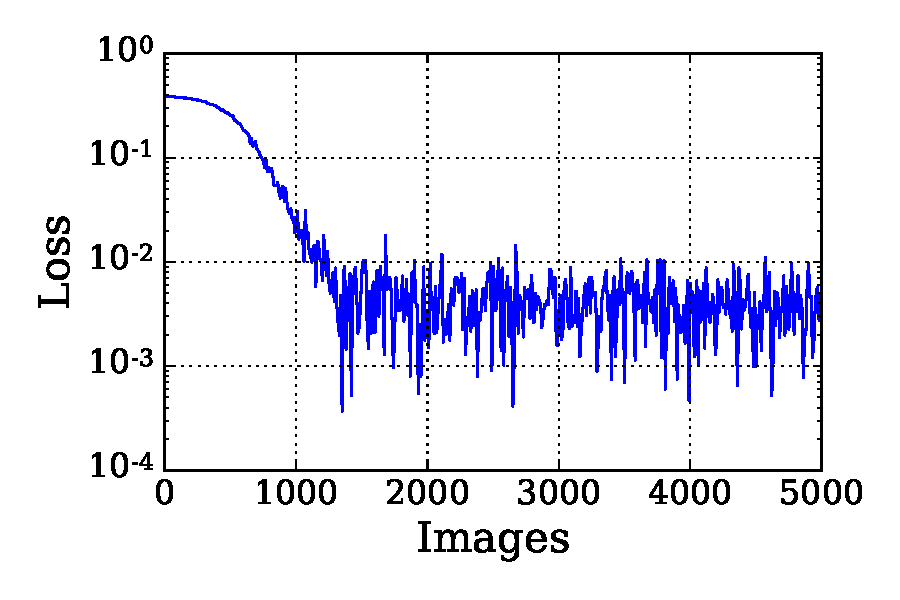
\includegraphics[width=\textwidth]{pics_sdlm/03_exp_SAE_noise_long/exp2_mse_nons.pdf}
		\caption{Loss of Exp2}
	\end{subfigure}
	\caption{Weights and firing rates of visible and hidden units change during training of the reconstruction tests of spiking AE with Solution 2. 
		Experiments 1) 10 visible units fully connected to 10 hidden units with Poisson spike trains of 100~Hz which lasted 100~ms; 2) same network fed with 10 Poisson spike trains of firing rate ranging from 10~Hz to 100~Hz.}
	\label{fig:sol2_ae}
\end{figure}

\begin{figure}
	\centering
	\begin{subfigure}[t]{0.48\textwidth}
		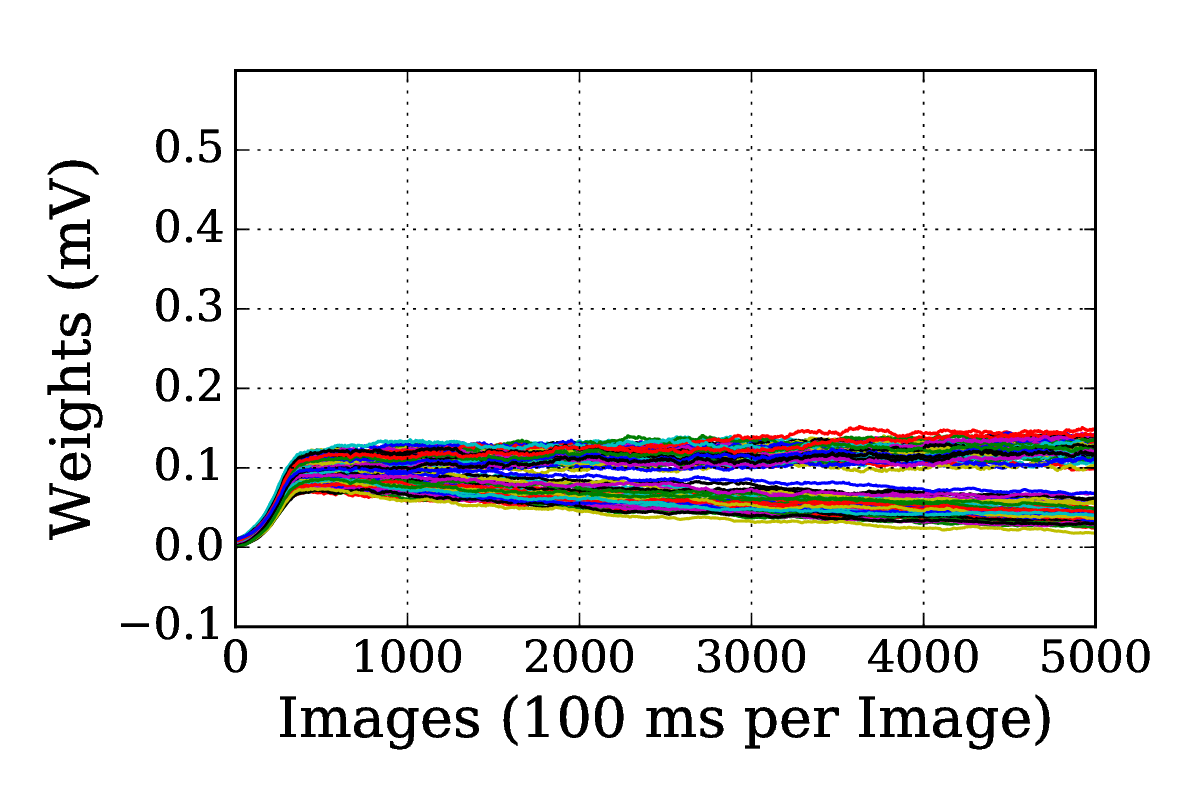
\includegraphics[width=\textwidth]{pics_sdlm/13_exp_SRBM_noise_long/exp1_weights_s.png}
		\caption{Weights of Exp1}
	\end{subfigure}
	\begin{subfigure}[t]{0.48\textwidth}
		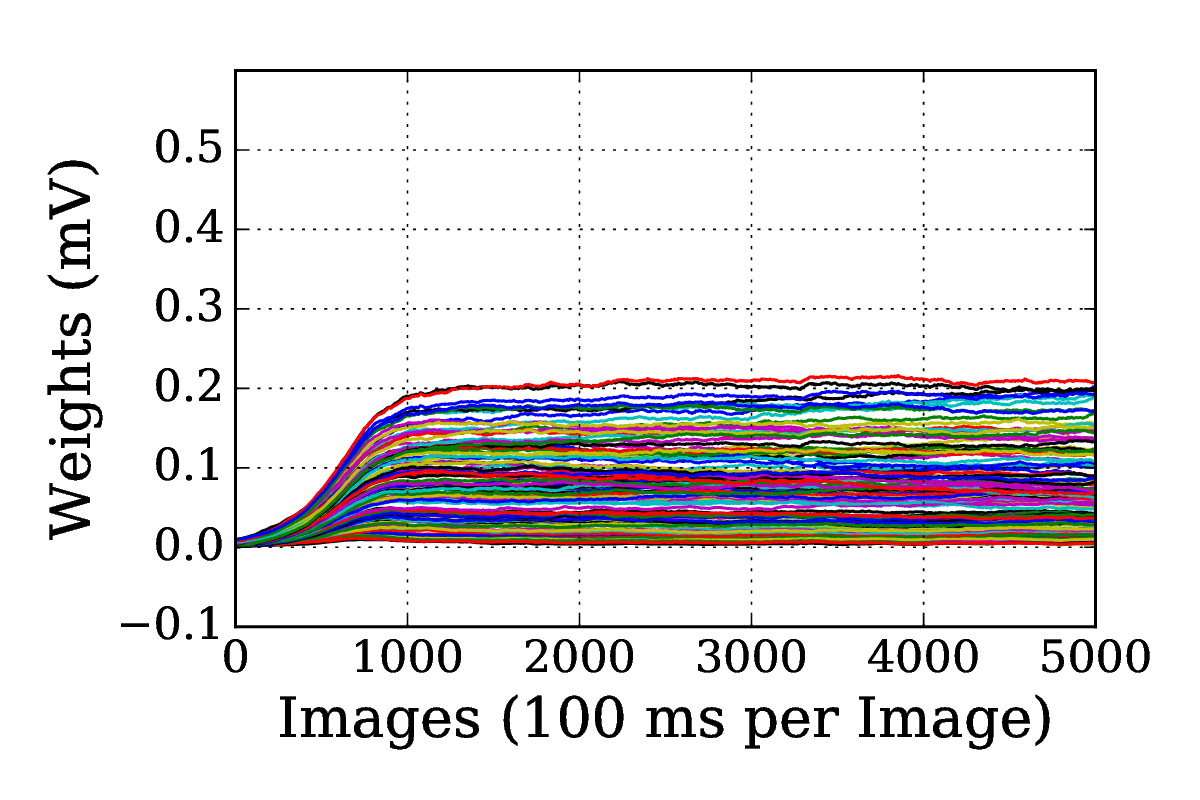
\includegraphics[width=\textwidth]{pics_sdlm/13_exp_SRBM_noise_long/exp2_weights_s.png}
		\caption{Weights of Exp2}
	\end{subfigure}
	\begin{subfigure}[t]{0.48\textwidth}
		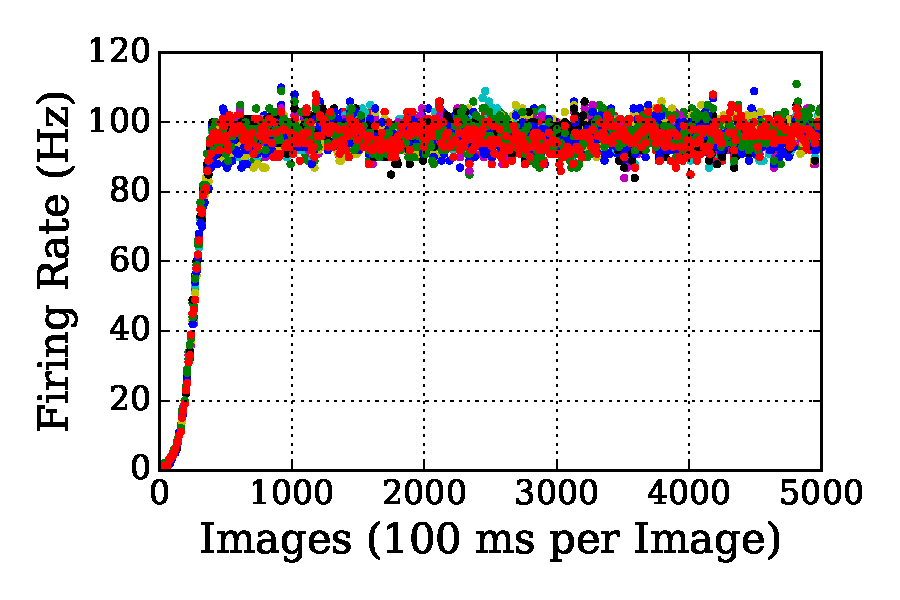
\includegraphics[width=\textwidth]{pics_sdlm/13_exp_SRBM_noise_long/exp1_recon_s.pdf}
		\caption{Reconstruction of visible units in Exp1}
	\end{subfigure}
	\begin{subfigure}[t]{0.48\textwidth}
		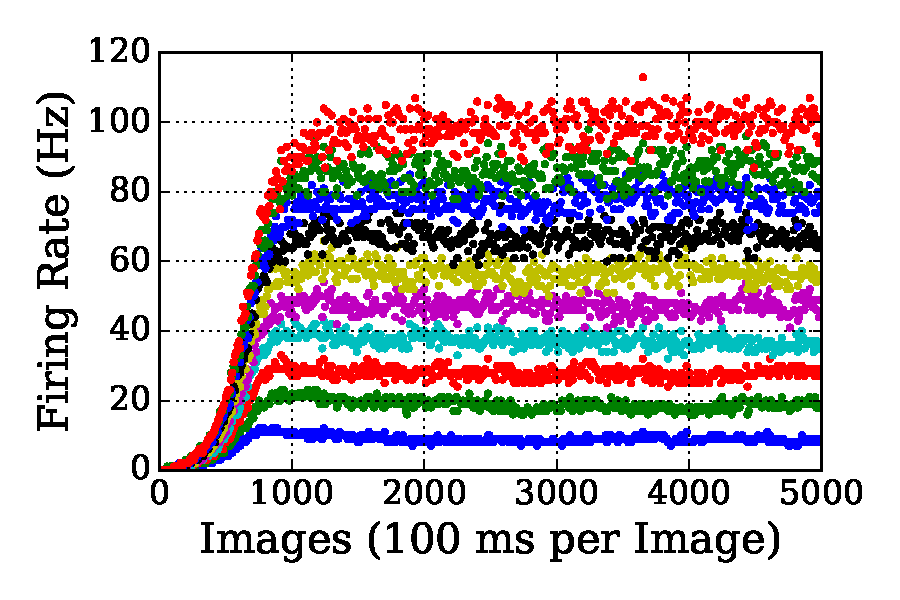
\includegraphics[width=\textwidth]{pics_sdlm/13_exp_SRBM_noise_long/exp2_recon_s.pdf}
		\caption{Reconstruction of visible units in Exp2}
	\end{subfigure}\\
	\begin{subfigure}[t]{0.48\textwidth}
		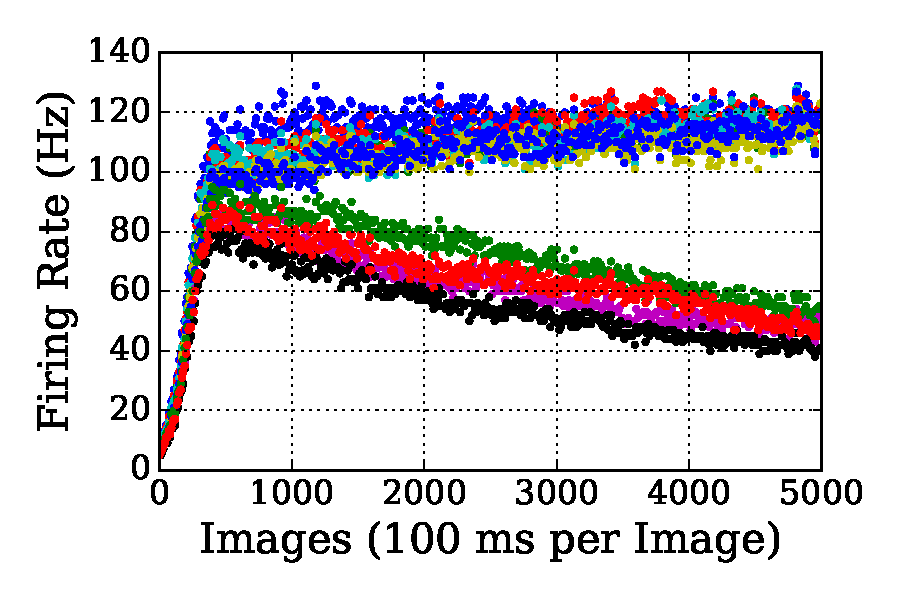
\includegraphics[width=\textwidth]{pics_sdlm/13_exp_SRBM_noise_long/exp1_hid_s.pdf}
		\caption{Output of hidden units in Exp1}
	\end{subfigure}
	\begin{subfigure}[t]{0.48\textwidth}
		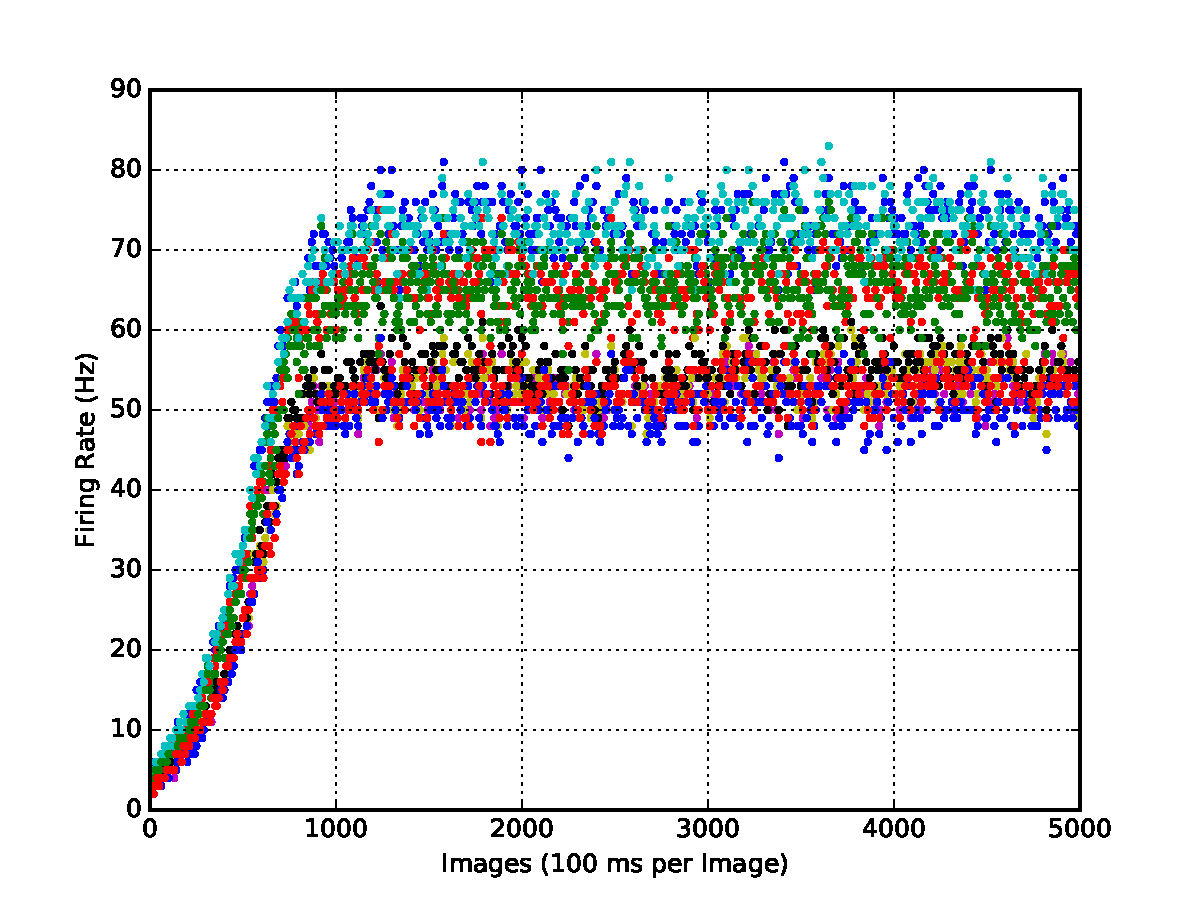
\includegraphics[width=\textwidth]{pics_sdlm/13_exp_SRBM_noise_long/exp2_hid_s.pdf}
		\caption{Output of hidden units in Exp2}
	\end{subfigure}\\
	\begin{subfigure}[t]{0.48\textwidth}
		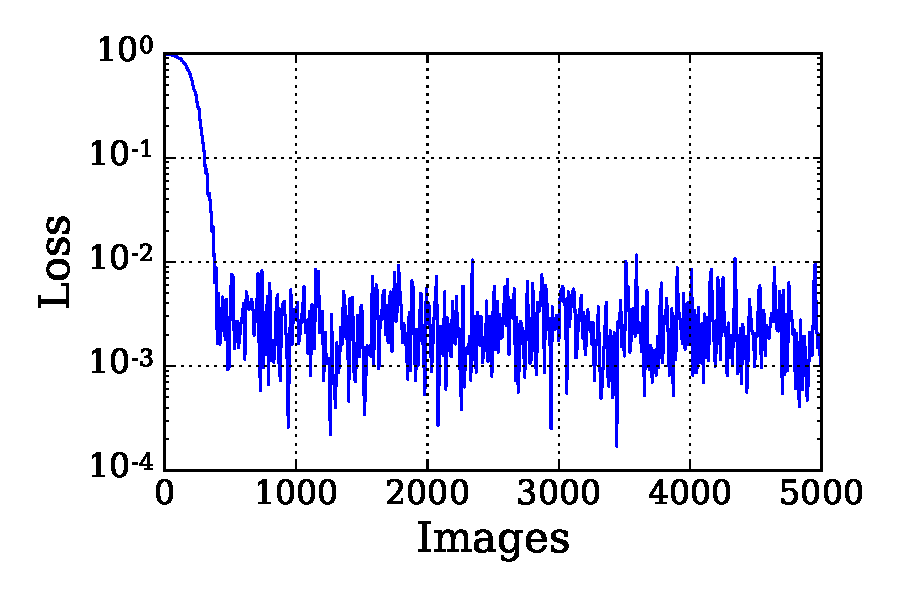
\includegraphics[width=\textwidth]{pics_sdlm/13_exp_SRBM_noise_long/exp1_mse_nons.pdf}
		\caption{Loss of Exp1}
	\end{subfigure}
	\begin{subfigure}[t]{0.48\textwidth}
		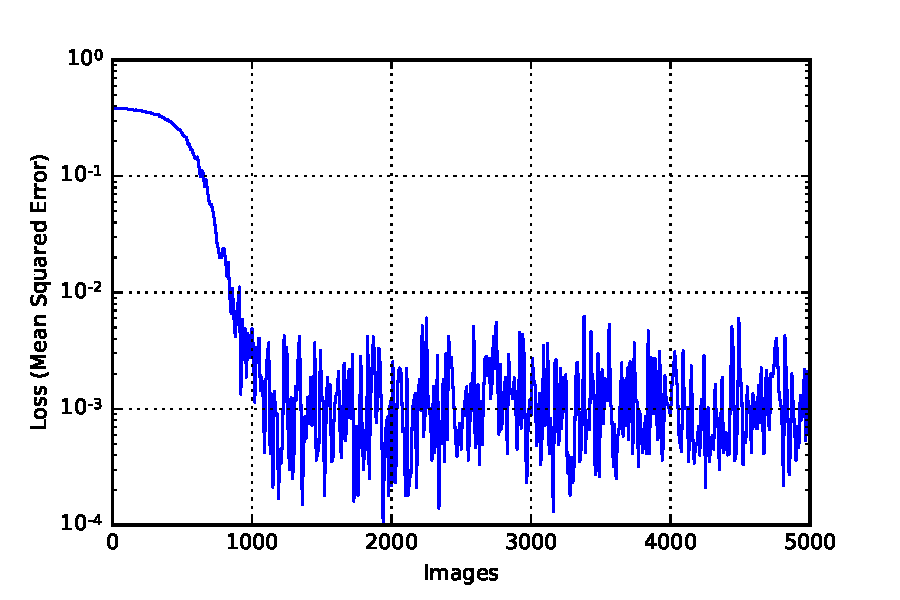
\includegraphics[width=\textwidth]{pics_sdlm/13_exp_SRBM_noise_long/exp2_mse_nons.pdf}
		\caption{Loss of Exp2}
	\end{subfigure}
	\caption{Weights and firing rates of visible and hidden units change during training of the reconstruction tests of spiking RBM with Solution~2. 
		Experiments 1) 10 visible units fully connected to 10 hidden units with Poisson spike trains of 100~Hz which lasted 100~ms; 2) same network fed with 10 Poisson spike trains of firing rate ranging from 10~Hz to 100~Hz.}
	\label{fig:sol2_rbm}
\end{figure}

\begin{figure}
	\centering
	\begin{subfigure}[t]{0.48\textwidth}
		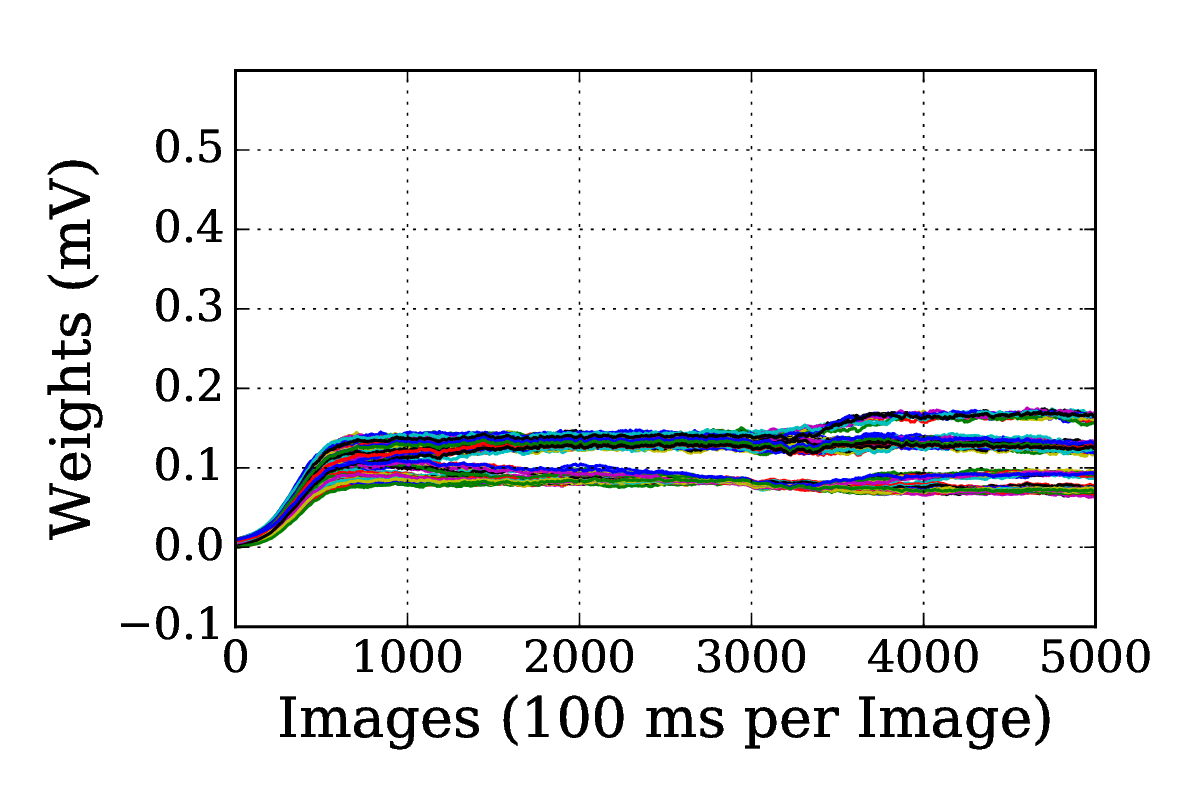
\includegraphics[width=\textwidth]{pics_sdlm/05_exp_SAE_teach_long/exp1_weights_s.png}
		\caption{Weights of Exp1}
	\end{subfigure}
	\begin{subfigure}[t]{0.48\textwidth}
		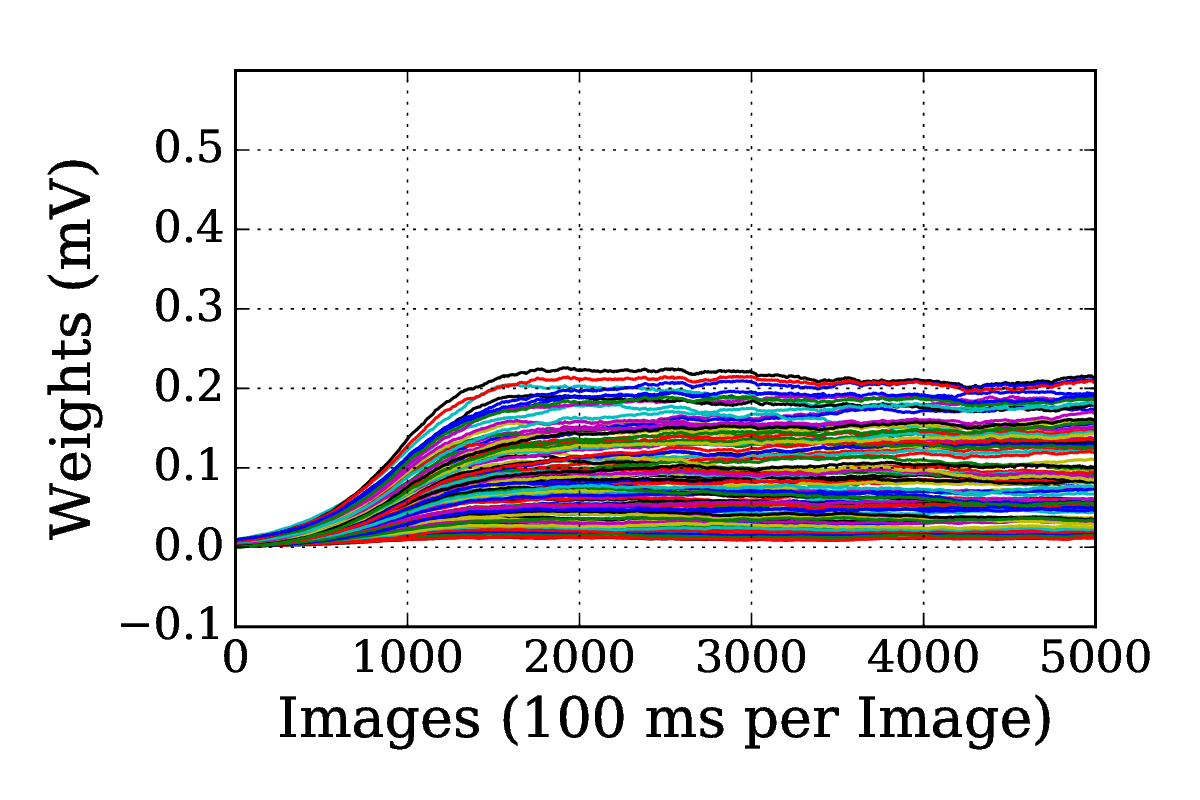
\includegraphics[width=\textwidth]{pics_sdlm/05_exp_SAE_teach_long/exp2_weights_s.png}
		\caption{Weights of Exp2}
	\end{subfigure}
	\begin{subfigure}[t]{0.48\textwidth}
		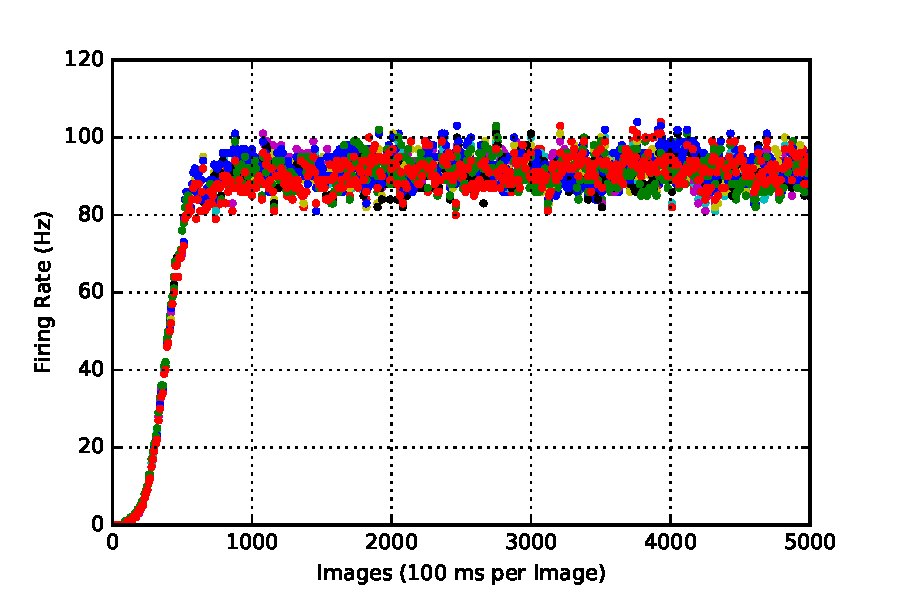
\includegraphics[width=\textwidth]{pics_sdlm/05_exp_SAE_teach_long/exp1_recon_s.pdf}
		\caption{Reconstruction of visible units in Exp1}
	\end{subfigure}
	\begin{subfigure}[t]{0.48\textwidth}
		\includegraphics[width=\textwidth]{pics_sdlm/05_exp_SAE_teach_long/exp2_recon_s.pdf}
		\caption{Reconstruction of visible units in Exp2}
	\end{subfigure}\\
	\begin{subfigure}[t]{0.48\textwidth}
		\includegraphics[width=\textwidth]{pics_sdlm/05_exp_SAE_teach_long/exp1_hid_s.pdf}
		\caption{Output of hidden units in Exp1}
	\end{subfigure}
	\begin{subfigure}[t]{0.48\textwidth}
		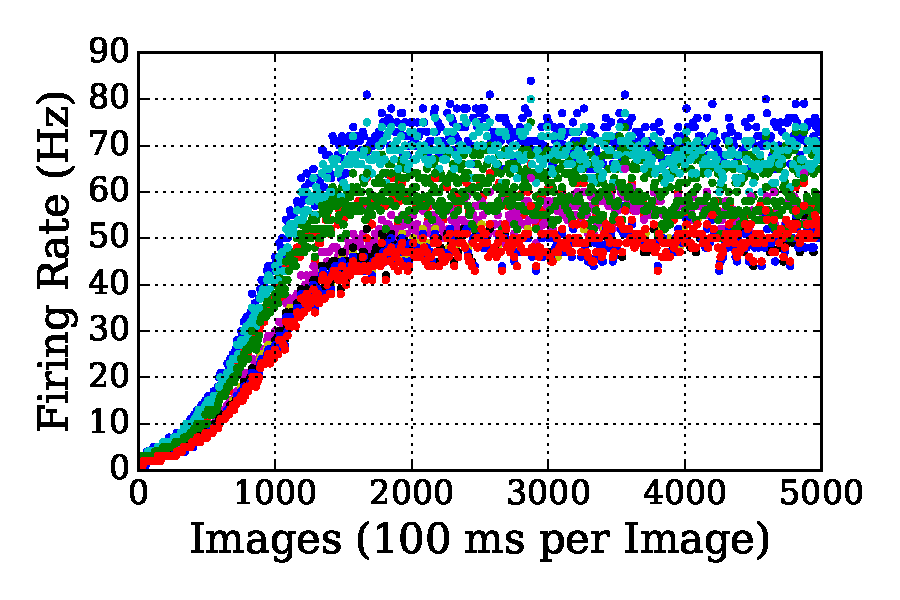
\includegraphics[width=\textwidth]{pics_sdlm/05_exp_SAE_teach_long/exp2_hid_s.pdf}
		\caption{Output of hidden units in Exp2}
	\end{subfigure}\\
	\begin{subfigure}[t]{0.48\textwidth}
		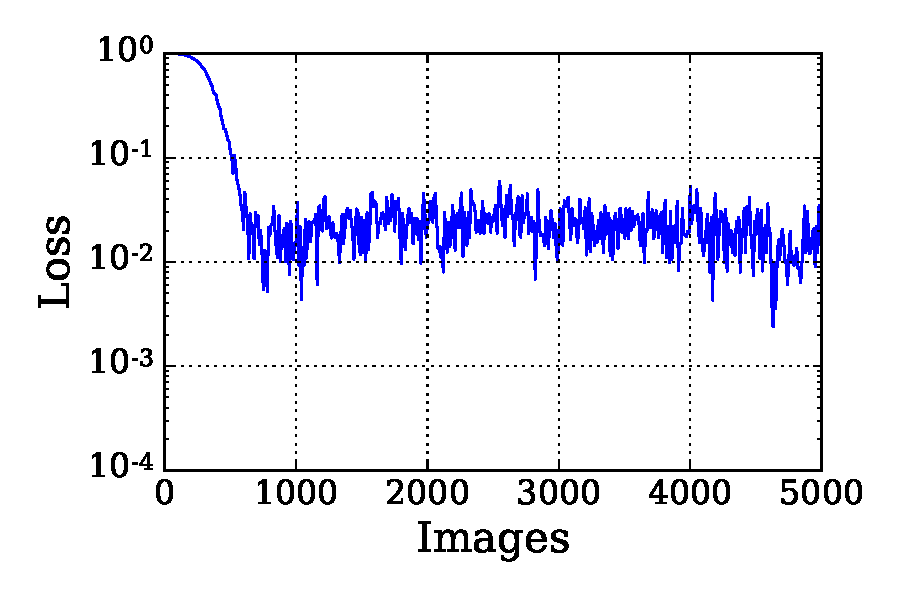
\includegraphics[width=\textwidth]{pics_sdlm/05_exp_SAE_teach_long/exp1_mse_nons.pdf}
		\caption{Loss of Exp1}
	\end{subfigure}
	\begin{subfigure}[t]{0.48\textwidth}
		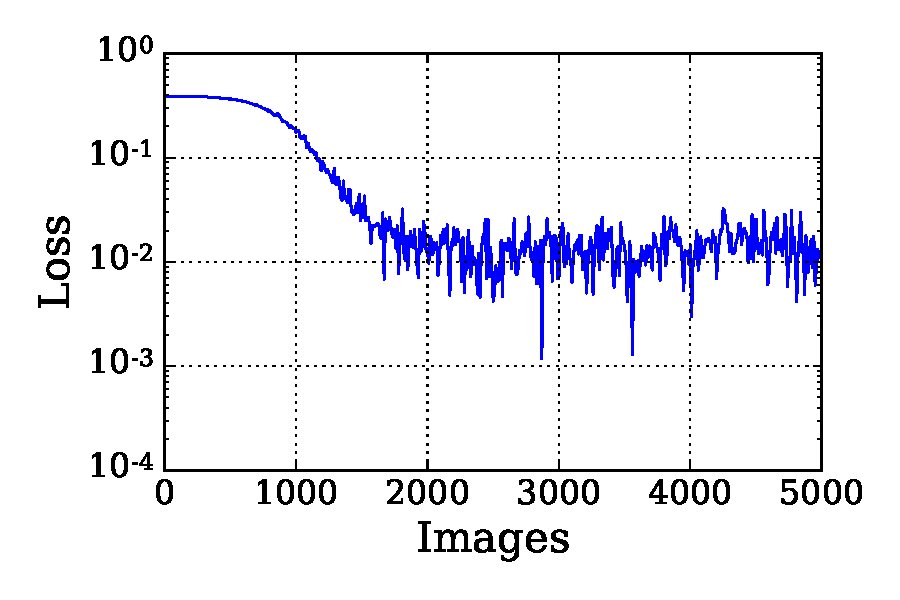
\includegraphics[width=\textwidth]{pics_sdlm/05_exp_SAE_teach_long/exp2_mse_nons.pdf}
		\caption{Loss of Exp2}
	\end{subfigure}
	\caption{Weights and firing rates of visible and hidden units change during training of the reconstruction tests of spiking AE with Solution~3. 
		Experiments 1) 10 visible units fully connected to 10 hidden units with Poisson spike trains of 100~Hz which lasted 100~ms; 2) same network fed with 10 Poisson spike trains of firing rate ranging from 10~Hz to 100~Hz.}
	\label{fig:sol3_ae}
\end{figure}

\begin{figure}
	\centering
	\begin{subfigure}[t]{0.48\textwidth}
		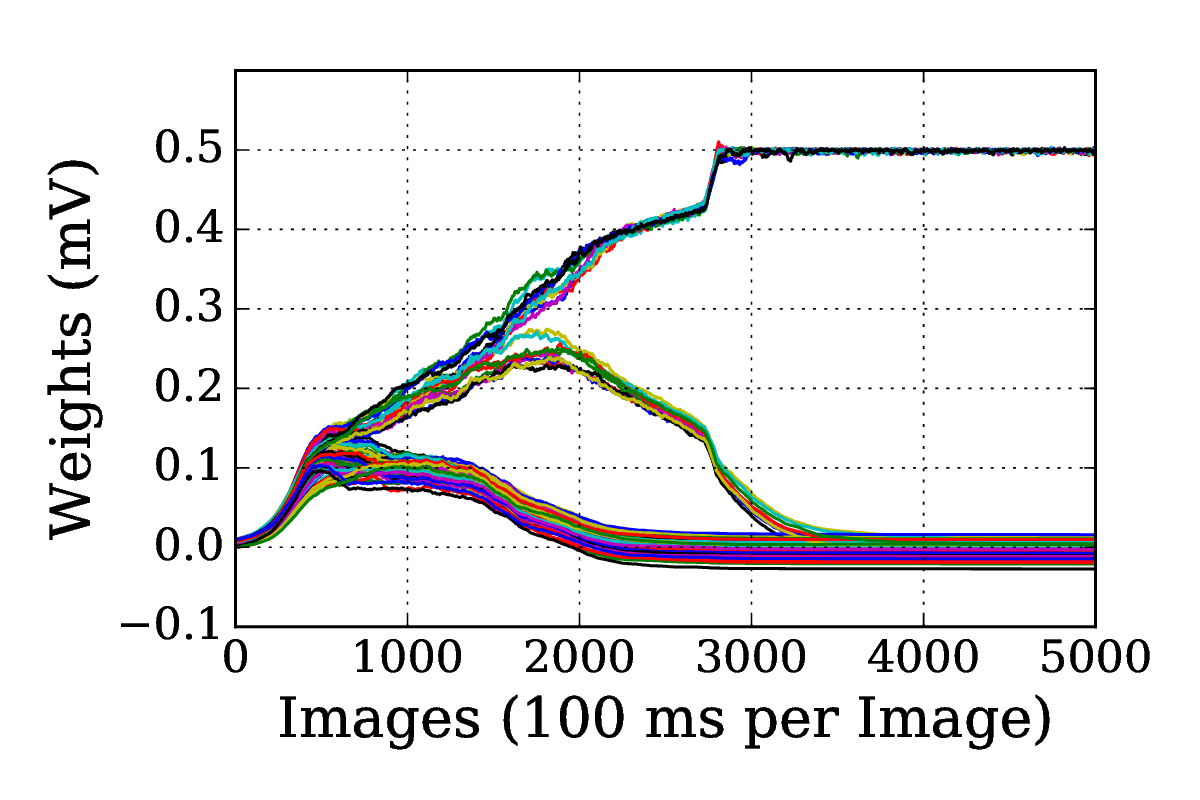
\includegraphics[width=\textwidth]{pics_sdlm/15_exp_SRBM_teach_long/exp1_weights_s.png}
		\caption{Weights of Exp1}
	\end{subfigure}
	\begin{subfigure}[t]{0.48\textwidth}
		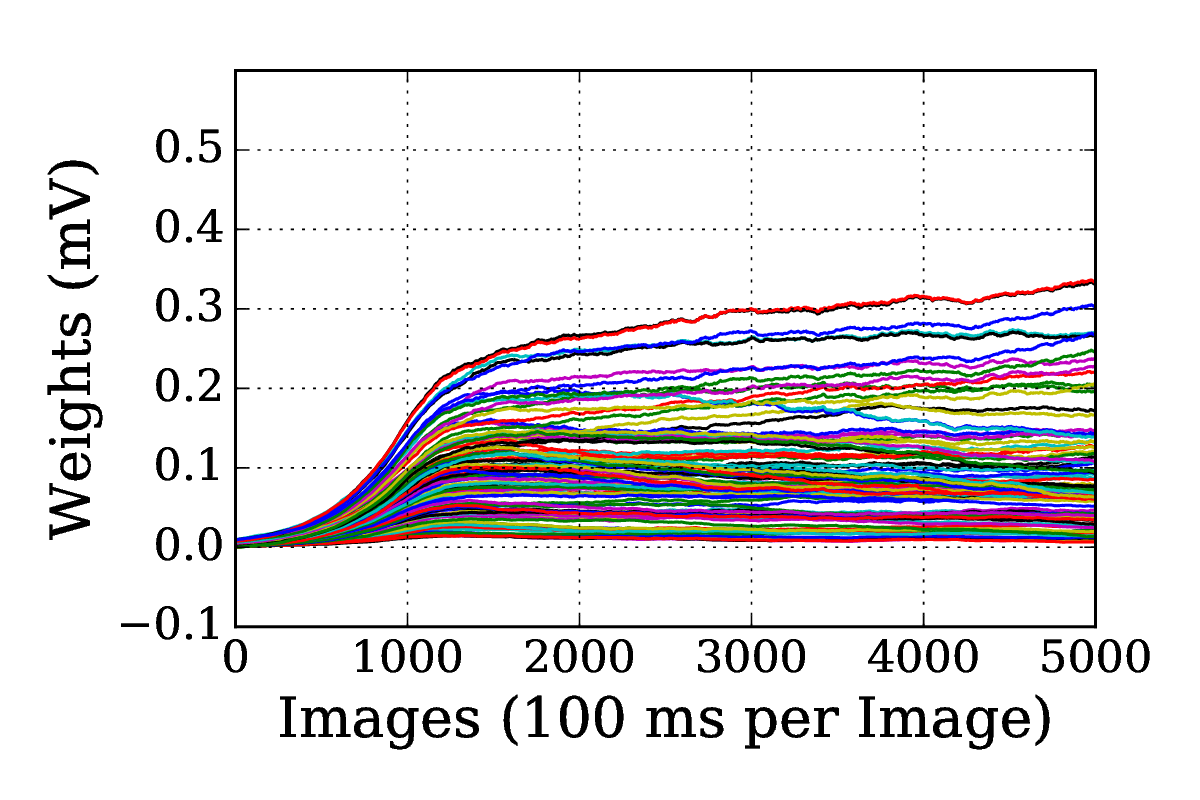
\includegraphics[width=\textwidth]{pics_sdlm/15_exp_SRBM_teach_long/exp2_weights_s.png}
		\caption{Weights of Exp2}
	\end{subfigure}
	\begin{subfigure}[t]{0.48\textwidth}
		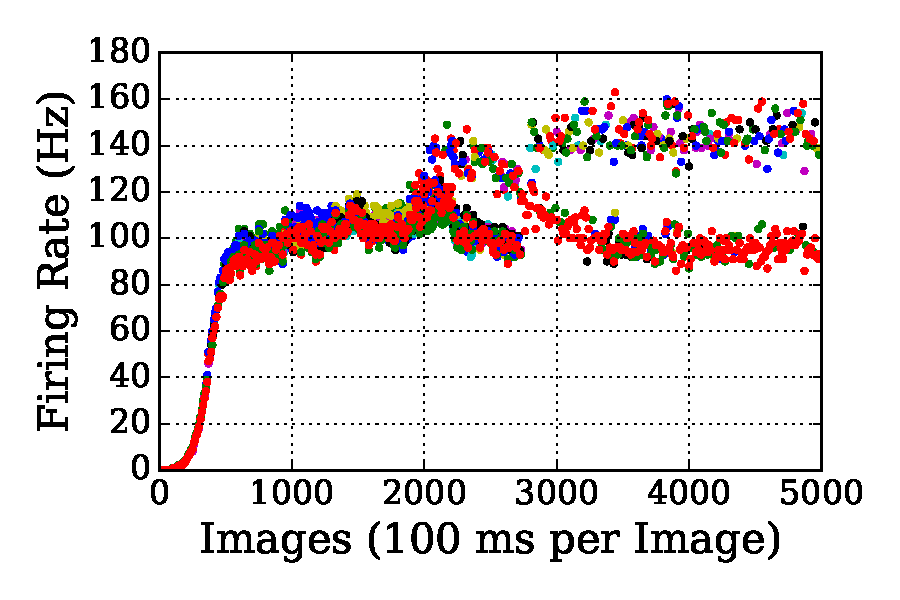
\includegraphics[width=\textwidth]{pics_sdlm/15_exp_SRBM_teach_long/exp1_recon_s.pdf}
		\caption{Reconstruction of visible units in Exp1}
	\end{subfigure}
	\begin{subfigure}[t]{0.48\textwidth}
		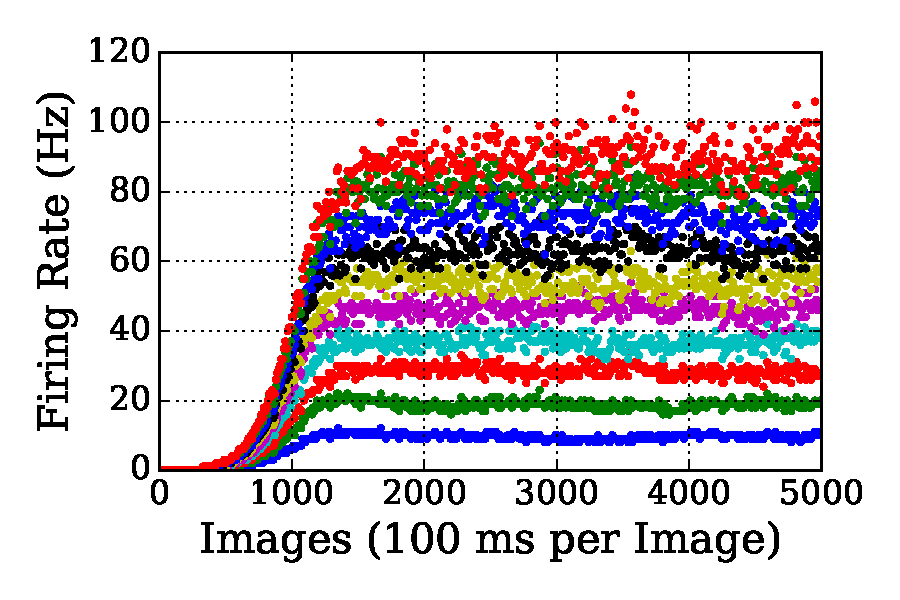
\includegraphics[width=\textwidth]{pics_sdlm/15_exp_SRBM_teach_long/exp2_recon_s.pdf}
		\caption{Reconstruction of visible units in Exp2}
	\end{subfigure}\\
	\begin{subfigure}[t]{0.48\textwidth}
		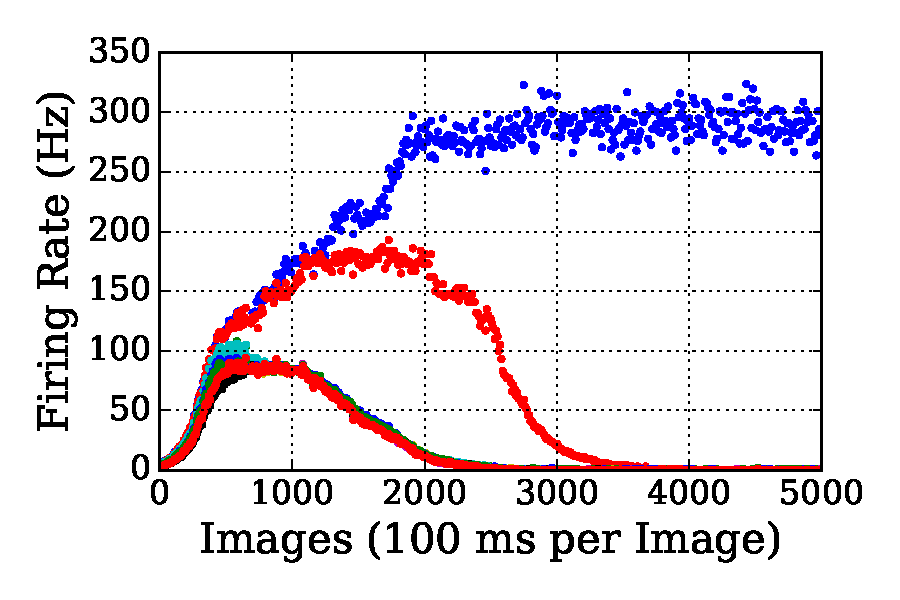
\includegraphics[width=\textwidth]{pics_sdlm/15_exp_SRBM_teach_long/exp1_hid_s.pdf}
		\caption{Output of hidden units in Exp1}
	\end{subfigure}
	\begin{subfigure}[t]{0.48\textwidth}
		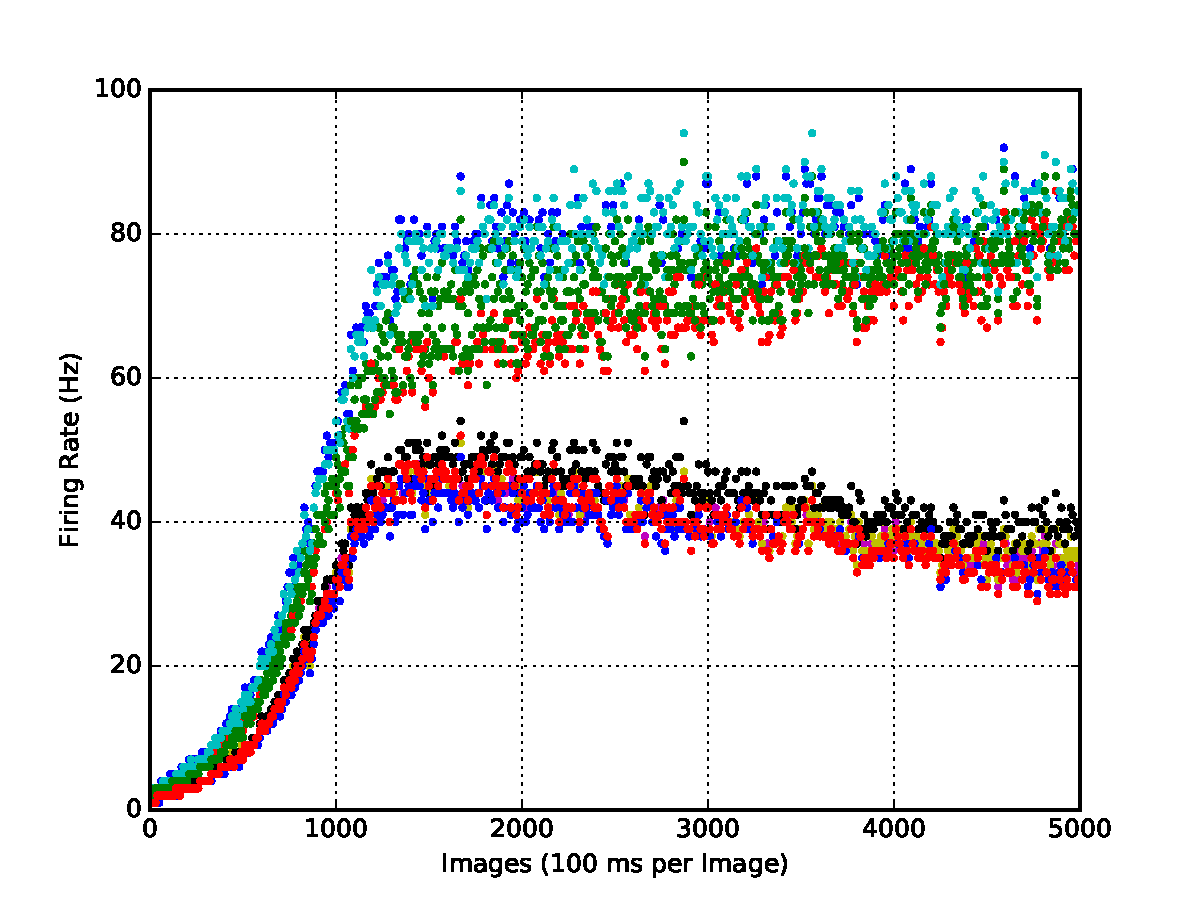
\includegraphics[width=\textwidth]{pics_sdlm/15_exp_SRBM_teach_long/exp2_hid_s.pdf}
		\caption{Output of hidden units in Exp2}
	\end{subfigure}\\
	\begin{subfigure}[t]{0.48\textwidth}
		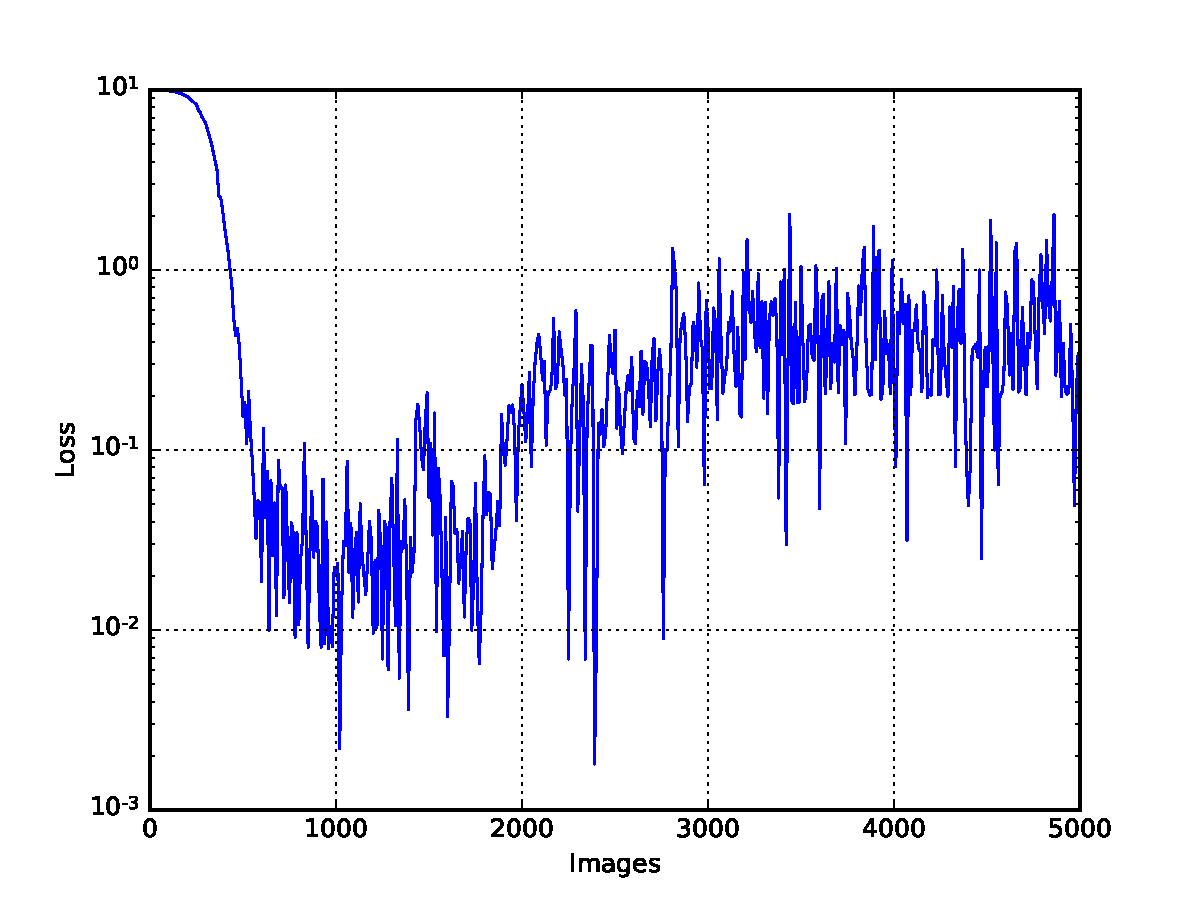
\includegraphics[width=\textwidth]{pics_sdlm/15_exp_SRBM_teach_long/exp1_mse_nons.pdf}
		\caption{Loss of Exp1}
	\end{subfigure}
	\begin{subfigure}[t]{0.48\textwidth}
		\includegraphics[width=\textwidth]{pics_sdlm/15_exp_SRBM_teach_long/exp2_mse_nons.pdf}
		\caption{Loss of Exp2}
	\end{subfigure}
	\caption{Weights and firing rates of visible and hidden units change during training of the reconstruction tests of spiking RBM with Solution~3. 
		Experiments 1) 10 visible units fully connected to 10 hidden units with Poisson spike trains of 100~Hz which lasted 100~ms; 2) same network fed with 10 Poisson spike trains of firing rate ranging from 10~Hz to 100~Hz.}
	\label{fig:sol3_rbm}
\end{figure}

\begin{figure}
	\centering
	\begin{subfigure}[t]{0.48\textwidth}
		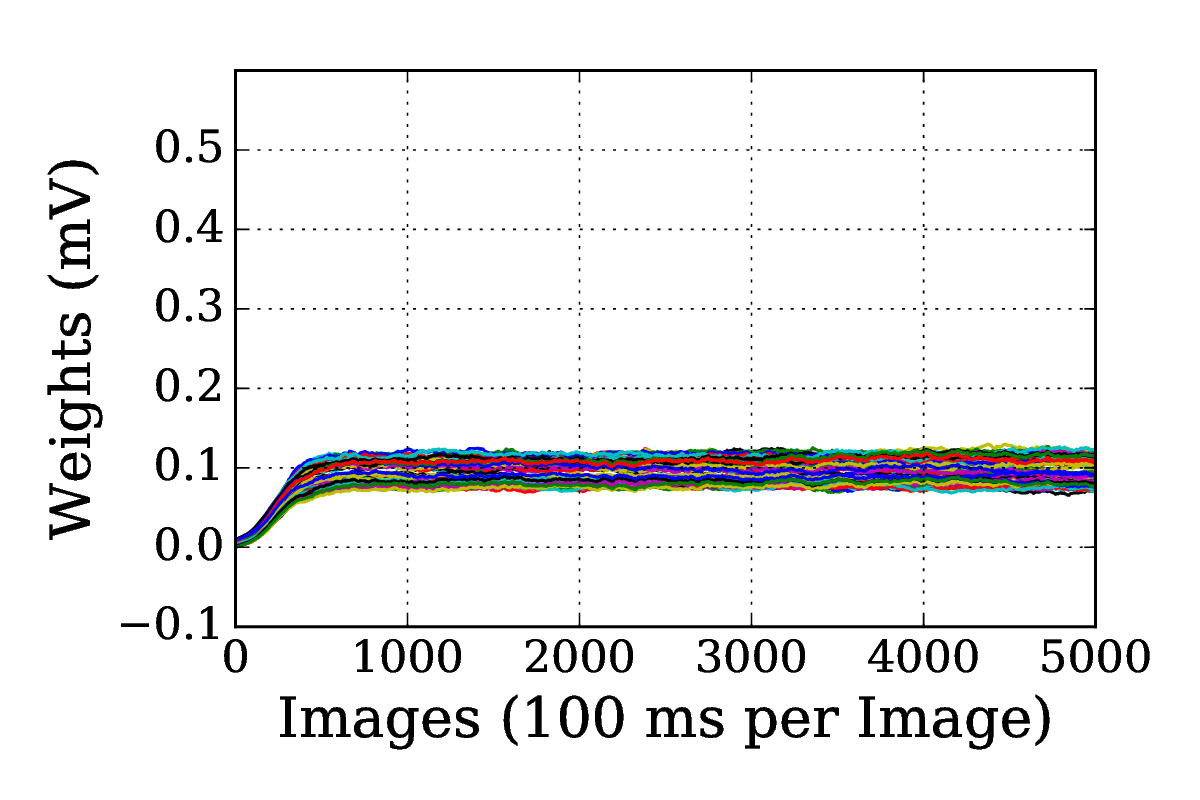
\includegraphics[width=\textwidth]{pics_sdlm/07_exp_SAE_all_long/exp1_weights_s.png}
		\caption{Weights of Exp1}
	\end{subfigure}
	\begin{subfigure}[t]{0.48\textwidth}
		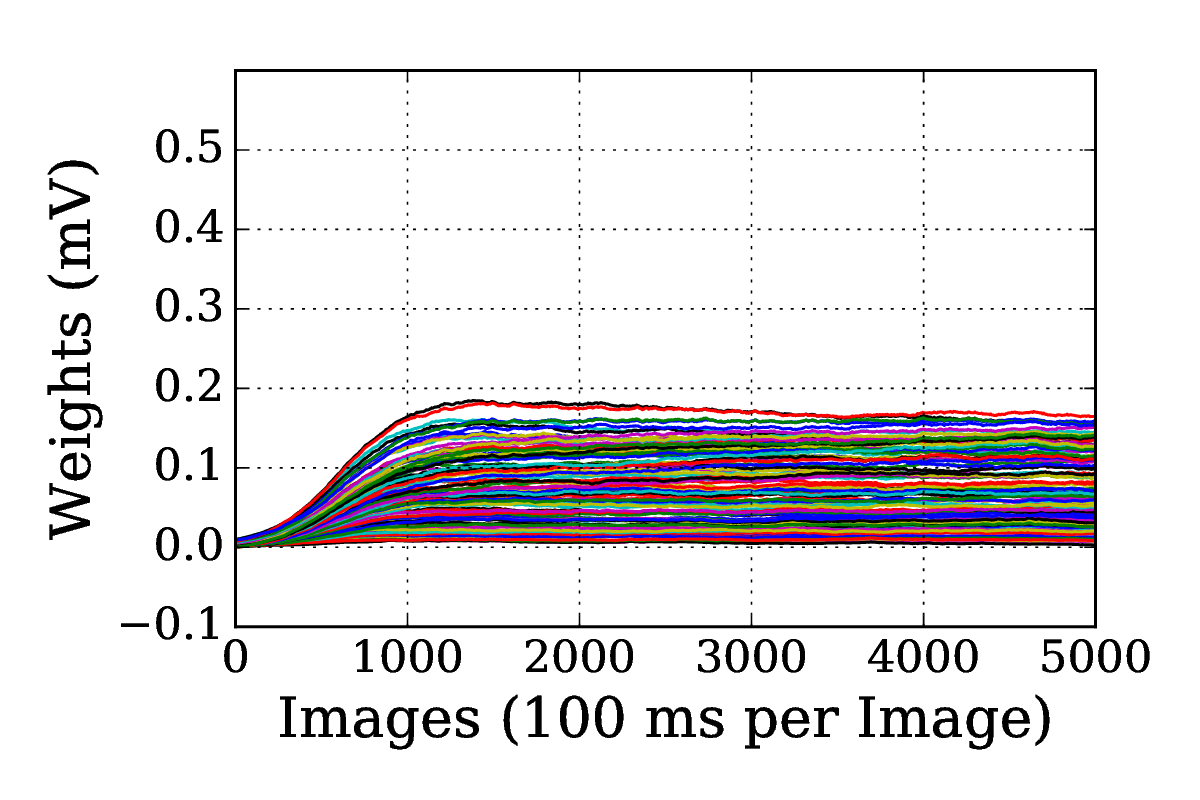
\includegraphics[width=\textwidth]{pics_sdlm/07_exp_SAE_all_long/exp2_weights_s.png}
		\caption{Weights of Exp2}
	\end{subfigure}
	\begin{subfigure}[t]{0.48\textwidth}
		\includegraphics[width=\textwidth]{pics_sdlm/07_exp_SAE_all_long/exp1_recon_s.pdf}
		\caption{Reconstruction of visible units in Exp1}
	\end{subfigure}
	\begin{subfigure}[t]{0.48\textwidth}
		\includegraphics[width=\textwidth]{pics_sdlm/07_exp_SAE_all_long/exp2_recon_s.pdf}
		\caption{Reconstruction of visible units in Exp2}
	\end{subfigure}\\
	\begin{subfigure}[t]{0.48\textwidth}
		\includegraphics[width=\textwidth]{pics_sdlm/07_exp_SAE_all_long/exp1_hid_s.pdf}
		\caption{Output of hidden units in Exp1}
	\end{subfigure}
	\begin{subfigure}[t]{0.48\textwidth}
		\includegraphics[width=\textwidth]{pics_sdlm/07_exp_SAE_all_long/exp2_hid_s.pdf}
		\caption{Output of hidden units in Exp2}
	\end{subfigure}\\
	\begin{subfigure}[t]{0.48\textwidth}
		\includegraphics[width=\textwidth]{pics_sdlm/07_exp_SAE_all_long/exp1_mse_nons.pdf}
		\caption{Loss of Exp1}
	\end{subfigure}
	\begin{subfigure}[t]{0.48\textwidth}
		\includegraphics[width=\textwidth]{pics_sdlm/07_exp_SAE_all_long/exp2_mse_nons.pdf}
		\caption{Loss of Exp2}
	\end{subfigure}
	\caption{Weights and firing rates of visible and hidden units change during training of the reconstruction tests of spiking AE with combined solutions. 
		Experiments 1) 10 visible units fully connected to 10 hidden units with Poisson spike trains of 100~Hz which lasted 100~ms; 2) same network fed with 10 Poisson spike trains of firing rate ranging from 10~Hz to 100~Hz.}
	\label{fig:sol4_ae}
\end{figure}

\begin{figure}
	\centering
	\begin{subfigure}[t]{0.48\textwidth}
		\includegraphics[width=\textwidth]{pics_sdlm/17_exp_SRBM_all_long/exp1_weights_s.png}
		\caption{Weights of Exp1}
	\end{subfigure}
	\begin{subfigure}[t]{0.48\textwidth}
		\includegraphics[width=\textwidth]{pics_sdlm/17_exp_SRBM_all_long/exp2_weights_s.png}
		\caption{Weights of Exp2}
	\end{subfigure}
	\begin{subfigure}[t]{0.48\textwidth}
		\includegraphics[width=\textwidth]{pics_sdlm/17_exp_SRBM_all_long/exp1_recon_s.pdf}
		\caption{Reconstruction of visible units in Exp1}
	\end{subfigure}
	\begin{subfigure}[t]{0.48\textwidth}
		\includegraphics[width=\textwidth]{pics_sdlm/17_exp_SRBM_all_long/exp2_recon_s.pdf}
		\caption{Reconstruction of visible units in Exp2}
	\end{subfigure}\\
	\begin{subfigure}[t]{0.48\textwidth}
		\includegraphics[width=\textwidth]{pics_sdlm/17_exp_SRBM_all_long/exp1_hid_s.pdf}
		\caption{Output of hidden units in Exp1}
	\end{subfigure}
	\begin{subfigure}[t]{0.48\textwidth}
		\includegraphics[width=\textwidth]{pics_sdlm/17_exp_SRBM_all_long/exp2_hid_s.pdf}
		\caption{Output of hidden units in Exp2}
	\end{subfigure}\\
	\begin{subfigure}[t]{0.48\textwidth}
		\includegraphics[width=\textwidth]{pics_sdlm/17_exp_SRBM_all_long/exp1_mse_nons.pdf}
		\caption{Loss of Exp1}
	\end{subfigure}
	\begin{subfigure}[t]{0.48\textwidth}
		\includegraphics[width=\textwidth]{pics_sdlm/17_exp_SRBM_all_long/exp2_mse_nons.pdf}
		\caption{Loss of Exp2}
	\end{subfigure}
	\caption{Weights and firing rates of visible and hidden units change during training of the reconstruction tests of spiking RBM with combined solutions. 
		Experiments 1) 10 visible units fully connected to 10 hidden units with Poisson spike trains of 100~Hz which lasted 100~ms; 2) same network fed with 10 Poisson spike trains of firing rate ranging from 10~Hz to 100~Hz.}
	\label{fig:sol4_rbm}
\end{figure}

%
\begin{figure}
	\centering
	\begin{subfigure}[c]{0.48\textwidth}\raggedleft
		\myrowlabel{Orignal SAE}
		\raisebox{-.5\height}{\includegraphics[width=.9\textwidth]
			{pics_sdlm/60_exp_SAE_Orig/exp2_weights_s.png}}\\
		\myrowlabel{S1}
		\raisebox{-.5\height}{\includegraphics[width=.9\textwidth]
			{pics_sdlm/61_exp_SAE_Orig_long/exp2_weights_s.png}}\\
		\myrowlabel{S2}
		\raisebox{-.5\height}{\includegraphics[width=.9\textwidth]
			{pics_sdlm/63_exp_SAE_noise_long/exp2_weights_s.png}}
		\myrowlabel{S3}
		\raisebox{-.5\height}{\includegraphics[width=.9\textwidth]
			{pics_sdlm/65_exp_SAE_teach_long/exp2_weights_s.png}}\\
		\myrowlabel{S4}
		\raisebox{-.5\height}{\includegraphics[width=.9\textwidth]
			{pics_sdlm/67_exp_SAE_all_long/exp2_weights_s.png}}
		\caption{Exp2 Weights}
	\end{subfigure}%
	\hspace{1em}
	\begin{subfigure}[c]{0.48\textwidth}\raggedleft
		\raisebox{-.5\height}{\includegraphics[width=.9\textwidth]
			{pics_sdlm/60_exp_SAE_Orig/exp2_mse_nons.pdf}}\\
		\raisebox{-.5\height}{\includegraphics[width=.9\textwidth]
			{pics_sdlm/61_exp_SAE_Orig_long/exp2_mse_nons.pdf}}\\
		\raisebox{-.5\height}{\includegraphics[width=.9\textwidth]
			{pics_sdlm/63_exp_SAE_noise_long/exp2_mse_nons.pdf}}
		\raisebox{-.5\height}{\includegraphics[width=.9\textwidth]
			{pics_sdlm/65_exp_SAE_teach_long/exp2_mse_nons.pdf}}\\
		\raisebox{-.5\height}{\includegraphics[width=.9\textwidth]
			{pics_sdlm/67_exp_SAE_all_long/exp2_mse_nons.pdf}}
		\caption{Exp2 Loss}
	\end{subfigure}%
	\caption{Comparisons of weights and loss of solutions for training SAE on Exp2 using LIF neurons: [S1] longer STDP window, [S2] noisy threshold, [S3] teaching signal, and [S4] combined solutions. 10 visible units fully connected to 10 hidden units with Poisson spike trains of firing rate ranging from 10~Hz to 100~Hz.}
	\label{fig:LIF_sae}
\end{figure}

\begin{figure}
	\centering
	\begin{subfigure}[c]{0.48\textwidth}\raggedleft
		\myrowlabel{Orignal SRBM}
		\raisebox{-.5\height}{\includegraphics[width=.9\textwidth]
			{pics_sdlm/70_exp_SRBM_Orig/exp2_weights_s.png}}\\
		\myrowlabel{S1}
		\raisebox{-.5\height}{\includegraphics[width=.9\textwidth]
			{pics_sdlm/71_exp_SRBM_Orig_long/exp2_weights_s.png}}\\
		\myrowlabel{S2}
		\raisebox{-.5\height}{\includegraphics[width=.9\textwidth]
			{pics_sdlm/73_exp_SRBM_noise_long/exp2_weights_s.png}}
		\myrowlabel{S3}
		\raisebox{-.5\height}{\includegraphics[width=.9\textwidth]
			{pics_sdlm/75_exp_SRBM_teach_long/exp2_weights_s.png}}\\
		\myrowlabel{S4}
		\raisebox{-.5\height}{\includegraphics[width=.9\textwidth]
			{pics_sdlm/77_exp_SRBM_all_long/exp2_weights_s.png}}
		\caption{Exp2 Weights}
	\end{subfigure}%
	\hspace{1em}
	\begin{subfigure}[c]{0.48\textwidth}\raggedleft
		\raisebox{-.5\height}{\includegraphics[width=.9\textwidth]
			{pics_sdlm/70_exp_SRBM_Orig/exp2_mse_nons.pdf}}\\
		\raisebox{-.5\height}{\includegraphics[width=.9\textwidth]
			{pics_sdlm/71_exp_SRBM_Orig_long/exp2_mse_nons.pdf}}\\
		\raisebox{-.5\height}{\includegraphics[width=.9\textwidth]
			{pics_sdlm/73_exp_SRBM_noise_long/exp2_mse_nons.pdf}}
		\raisebox{-.5\height}{\includegraphics[width=.9\textwidth]
			{pics_sdlm/75_exp_SRBM_teach_long/exp2_mse_nons.pdf}}\\
		\raisebox{-.5\height}{\includegraphics[width=.9\textwidth]
			{pics_sdlm/77_exp_SRBM_all_long/exp2_mse_nons.pdf}}
		\caption{Exp2 Loss}
	\end{subfigure}%
	\caption{Comparisons of weights and loss of solutions for training SRBM on Exp2 using LIF neurons: [S1] longer STDP window, [S2] noisy threshold, [S3] teaching signal, and [S4] combined solutions. 10 visible units fully connected to 10 hidden units with Poisson spike trains of firing rate ranging from 10~Hz to 100~Hz.}
	\label{fig:LIF_srbm}
\end{figure}


\begin{figure}
	\centering
	\includegraphics[width=\textwidth]{pics_sdlm/22_MNIST_AE/2_60000_0.pdf}
	\caption{Trained weights after 3 epochs of MNIST training using AE, same as Figure~\ref{fig:weights_ae}(a)}
	\label{fig:weights_ae1}
\end{figure}

\begin{figure}
	\centering
	\includegraphics[width=\textwidth]{pics_sdlm/23_MNIST_AE_noise/2_60000_0.pdf}
	\caption{Trained weights after 3 epochs of MNIST training using AE-NI, same as Figure~\ref{fig:weights_ae}(b).}
	\label{fig:weights_ae2}
\end{figure}

\begin{figure}
	\centering
	\includegraphics[width=\textwidth]{pics_sdlm/40_MNIST_SAE_original/2_60000_0.pdf}
	\caption{Trained weights after 3 epochs of MNIST training using Original SAE, same as Figure~\ref{fig:weights_ae}(c).}
	\label{fig:weights_ae3}
\end{figure}

\begin{figure}
	\centering
	\includegraphics[width=\textwidth]{pics_sdlm/42_MNIST_SAE_noise/2_60000_0.pdf}
	\caption{Trained weights after 3 epochs of MNIST training using SAE-S2, same as Figure~\ref{fig:weights_ae}(d)}
	\label{fig:weights_ae4}
\end{figure}

\begin{figure}
	\centering
	\includegraphics[width=\textwidth]{pics_sdlm/41_MNIST_SAE_teach/2_60000_0.pdf}
	\caption{Trained weights after 3 epochs of MNIST training using SAE-S3, same as Figure~\ref{fig:weights_ae}(e).}
	\label{fig:weights_ae5}
\end{figure}

\begin{figure}
	\centering
	\includegraphics[width=\textwidth]{pics_sdlm/43_MNIST_SAE_all/2_60000_0.pdf}
	\caption{Trained weights after 3 epochs of MNIST training using SAE-S4, same as Figure~\ref{fig:weights_ae}(f).}
	\label{fig:weights_ae6}
\end{figure}


\begin{figure}
	\centering
	\includegraphics[width=\textwidth]{pics_sdlm/32_MNIST_RBM/2_60000_0.pdf}
	\caption{Trained weights after 3 epochs of MNIST training using nRBM, same as Figure~\ref{fig:weights_rbm}(a)}
	\label{fig:weights_rbm1}
\end{figure}

\begin{figure}
	\centering
	\includegraphics[width=\textwidth]{pics_sdlm/33_MNIST_RBM_noise/2_60000_0.pdf}
	\caption{Trained weights after 3 epochs of MNIST training using nRBM-NI, same as Figure~\ref{fig:weights_rbm}(b).}
	\label{fig:weights_rbm2}
\end{figure}

\clearpage
\begin{figure}
	\centering
	\includegraphics[width=\textwidth]{pics_sdlm/50_MNIST_SRBM_original/2_60000_0.pdf}
	\caption{Trained weights after 3 epochs of MNIST training using Original SRBM, same as Figure~\ref{fig:weights_rbm}(c).}
	\label{fig:weights_rbm3}
\end{figure}

\begin{figure}
	\centering
	\includegraphics[width=\textwidth]{pics_sdlm/52_MNIST_SRBM_noise/2_60000_0.pdf}
	\caption{Trained weights after 3 epochs of MNIST training using SRBM-S2, same as Figure~\ref{fig:weights_rbm}(d)}
	\label{fig:weights_rbm4}
\end{figure}

\begin{figure}
	\centering
	\includegraphics[width=\textwidth]{pics_sdlm/51_MNIST_SRBM_teach/2_60000_0.pdf}
	\caption{Trained weights after 3 epochs of MNIST training using SRBM-S3, same as Figure~\ref{fig:weights_rbm}(e).}
	\label{fig:weights_rbm5}
\end{figure}

\begin{figure}
	\centering
	\includegraphics[width=\textwidth]{pics_sdlm/53_MNIST_SRBM_all/2_60000_0.pdf}
	\caption{Trained weights after 3 epochs of MNIST training using SRBM-S4, same as Figure~\ref{fig:weights_rbm}(f).}
	\label{fig:weights_rbm6}
\end{figure}



